% This is samplepaper.tex, a sample chapter demonstrating the
% LLNCS macro package for Springer Computer Science proceedings;
% Version 2.21 of 2022/01/12
%
\documentclass[runningheads]{llncs}
%
\usepackage[T1]{fontenc}
\usepackage{courier} %% Sets font for listing as Courier.
\usepackage{listings, xcolor}
\usepackage{hyperref}
% \lstset{
%     escapeinside={(*@}{@*)},          % if you want to add LaTeX within your code
% }
\usepackage{booktabs}
% T1 fonts will be used to generate the final print and online PDFs,
% so please use T1 fonts in your manuscript whenever possible.
% Other font encondings may result in incorrect characters.
%
\usepackage{graphicx}
% Used for displaying a sample figure. If possible, figure files should
% be included in EPS format.
%
% If you use the hyperref package, please uncomment the following two lines
% to display URLs in blue roman font according to Springer's eBook style:
%\usepackage{color}
%\renewcommand\UrlFont{\color{blue}\rmfamily}
%\urlstyle{rm}
%
\usepackage{listings, xcolor}
\definecolor{javapurple}{rgb}{0.5,0,0.35} % strings
\definecolor{linenumbergray}{rgb}{0.5,0.5,0.5}
\lstdefinestyle{Java-github}{
        basicstyle=\ttfamily\tiny,
        language=Java,
        commentstyle=\color{linenumbergray},
        stringstyle=\color{javapurple},
        keywordstyle=\color{red},
        morekeywords={@Test},
        morecomment=[s][\color{linenumbergray}]{/**}{*/},
        numbers=left,
        numberstyle=\tiny\color{linenumbergray},
        numbersep=2.5pt,
        xleftmargin=1em,
        moredelim=**[is][\color{javapurple}]{@h@}{@h@},
        morecomment=[f][{\btHL[fill=gitdel]}]-,
        morecomment=[f][{\btHL[fill=gitadd]}]+,
        breaklines = true,
        %escapeinside={(*@}{@*)}
}
\lstdefinestyle{prompt}{
     basicstyle=\ttfamily\tiny,
     language=Html,
     commentstyle=\color{linenumbergray},
     stringstyle=\color{javapurple},
     keywordstyle=\color{red},
     morekeywords={@Test},
     morecomment=[s][\color{linenumbergray}]{/**}{*/},
     numbers=left,
     numberstyle=\tiny\color{linenumbergray},
     numbersep=2.5pt,
     xleftmargin=1em,
     moredelim=**[is][\color{javapurple}]{@h@}{@h@},
     morecomment=[f][{\btHL[fill=gitdel]}]-,
     morecomment=[f][{\btHL[fill=gitadd]}]+,
     breaklines = true, 
     %escapeinside={(*@}{@*)}
}
\begin{document}
%
\title{An approach for API synthesis using large language models}
%
%\titlerunning{Abbreviated paper title}
% If the paper title is too long for the running head, you can set
% an abbreviated paper title here
%
\author{Hua Zhong \and
Shan Jiang \and
Sarfraz Khurshid}
%
\authorrunning{Hua et al.}
% First names are abbreviated in the running head.
% If there are more than two authors, 'et al.' is used.
%
\institute{The University of Texas at Austin, Austin TX 78712, USA}
%
\maketitle              % typeset the header of the contribution
%

\newcommand{\NumTasks}{135}
\newcommand{\NumTasksCompletedOurApproach}{133}

\begin{abstract}
APIs play a pivotal role in modern software development by enabling seamless communication and integration between various systems, applications, and services. Component-based API synthesis is a form of program synthesis that constructs an API by assembling predefined components from a library. Existing API synthesis techniques typically implement dedicated search strategies over bounded spaces of possible implementations, which can be very large and time consuming to explore.
In this paper, we present a novel approach of using large language models (LLMs) in API synthesis.  LLMs offer a foundational technology to capture developer insights and provide an ideal framework for enabling more effective API synthesis.  We perform an experimental evaluation of our approach using \NumTasks~real-world programming tasks, and compare it with FrAngel, a state-of-the-art API synthesis tool.  The experimental results show that our approach completes \NumTasksCompletedOurApproach~of the tasks, and overall outperforms FrAngel. We believe LLMs provide a very useful foundation for tackling the problem of API synthesis, in particular, and program synthesis, in general.

% approach to synthesize complex APIs without the requirement of program components. We employ large language models as a foundational technology to encapsulate our insights within a framework for API synthesis. 

% We successfully evaluated our approach to synthesize complex APIs from realworld programming tasks. Moreover, our approach performs in par with a state-of-the-art API synthesis tool, despite not requiring the additional input of program components. 

\keywords{Component-based Synthesis \and Program Synthesis \and Large Language Models \and Complex APIs}.
\end{abstract}
%
%
%

\section{Introduction}
The increasing complexity of modern software systems has made the correct usage of APIs and dependent libraries a significant challenge for developers\cite{lamothe2021systematic}. Jungloid mining \cite{jungloid} highlights that even experienced developers often spend substantial time identifying a few relevant functions within a library. Similarly, Shi et al. \cite{frangel} observed that programmers frequently explore libraries to locate useful functions, which often need to be combined with intricate control structures, such as loops and conditions, to implement desired functionalities. These challenges complicate program synthesis, as they require not only knowledge of the library's components but also the integration of those components into coherent, functional code.

API synthesis is particularly demanding because it requires an understanding of the intended behavior, which is usually only known to the developer and often lacks formal documentation suitable for automated reasoning. While various specification methods exist - such as logical constraints \cite{10.1145/1993316.1993506,proveri} and executable specifications \cite{mimic,oguide} - synthesizing APIs using input-output examples has emerged as a user-friendly alternative\cite{frangel}. This approach allows developers to communicate intended functionality through input/output examples for synthesis programs. This method is especially beneficial for non-programmers, who can use examples to articulate their requirements without needing technical expertise \cite{stringio}.

Previous approaches to component-based synthesis often rely on domain-specific knowledge to address particular problem classes, such as string manipulation \cite{icmlpbe,stringio} or data transformations \cite{syndstrans,syntable}. And test-driven-synthesis\cite{testdriven} describe a general framework that leverages expert-written domain-specific languages (DSLs). While other approaches, such as loop free synthesis\cite{loopfree} and oracle guided synthesis \cite{oguide}, are domain-agnostic but depend on formal component specifications. But such methods requires knowledge of expected behavior, which may only be known to the developer and may not not exist in a formal language that supports automated reasoning. However, writing formal specifications for every component in software libraries is labor-intensive and often impractical. While these synthesis approaches for complex APIs handle various practical synthesis problems, they are largely limited to creating single basic blocks of code and do not readily handle multiple blocks in the presence of loops (or recursion) and complex tests. A key issue with handling multiple blocks is the very large size of the space of possible method sequences and their combinations.

More recent methods, such as SyPet\cite{sypet}, EdSynth\cite{Edsynth}, and FrAngel\cite{frangel}, have aimed to reduce reliance on DSLs or formal specifications by using black-box execution instead of reasoning about formal semantics. While SyPet struggles with synthesizing programs that involve complex control structures like loops and conditionals, FrAngel introduces a strategy using angelic conditions and EdSynth eliminate this problem by sketching. FrAngel first identifies promising program structures and then resolves the control flow through optimistic evaluation. By iteratively refining control flows that pass test cases, FrAngel succeeds in combining known behaviors with control structures to uncover more complex functionalities \cite{pnondet}. LooPy\cite{loopy} makes use of live execution, a technique that leverages the programmer as an oracle to step over incomplete parts of the loop, which also got rid of the dependence on DSL. However, programmers as oracles also makes LooPy rely on the programmer and cannot automatically synthesis APIs.


In this paper, we propose an approach that leverage LLMs with prompt engineering for systematic study of synthesizing complex APIs. LLMs have recently shown exceptional capabilities in tasks involving both natural language understanding and code synthesis \cite{li2023cctest,nam2024using,jiang2024generating}. Trained on large datasets, including extensive code repositories and documentation, LLMs possess an implicit understanding of programming syntax and semantics. These models can align user inputs with their pre-existing knowledge \cite{liu2024llm} and even address tasks that are uncommon in their training data \cite{schaeffer2024emergent}. Unlike previous synthesis methods, which often rely on domain-specific knowledge or predefined formal specifications, LLMs excel at managing complex, open-ended programming tasks. They can synthesis APIs based on natural language prompts and simple input/output examples, eliminating the need for explicit specifications or DSLs. Furthermore, LLMs handle intricate control structures such as loops and conditionals with ease, making them highly versatile and efficient. By directly interpreting developer intent through input/output examples, LLMs reduce the burden on developers, enabling rapid and adaptive solutions for diverse functionalities.

An exciting consequence of using LLMs is that our approach requires minimal user input (e.g., fewer test cases than FrAngel) compared to other methods and provides richer implementations that include meaningful variable names and comments. The user just provides a few simplified input/output examples and the API signature and LLMs can synthesis correct API. In contrast, previous work like FrAngel have to define a complete set of component API which is the search space. The rich training corpus of LLMs allow them to be used without explicitly having to include all relevant technical details, such as complete lists of allowed APIs (components) to use. Checking program correctness -- a non-trivial task -- is simplified through the use of simple input/out examples, which allow developers to validate that the generated API meets their intended requirements. Developing compelete test cases remains a challenging problem and prior program-by-example (PBE) methods have struggled with corner cases. Our evaluation demonstrates that LLMs, due to their extensive training data and their ability to infer intended functionality from API signature, can handle corner cases with just a few test cases. Our approach simplifies the synthesis process while maintaining reliability and accuracy, offering a practical and accessible solution for developers. Specifically, our approach synthesizes 133 correct APIs out of 135 benchmarks, outperforms previous state-of-the-art technique, FrAngel, in accuracy and readability. 

In addition, to ensure that our method has generalization ability, we use the evaluation dataset in FrAngel which covers different complexity of APIs in different scenario. Besides, we design our additional dataset of 15 new APIs that are not present in open-source projects, which ensures that LLMs are truly capable of synthesizing API implementations based on input/output examples rather than simply reproducing content in their large training set.

This paper makes the following contributions:

\begin{itemize}
    \item {\bf Approach}.  We present a novel approach to use LLMs to do API synthesis.  By combining prompt techniques such as assistant context, chain-of-thought prompting, few-shot learning, and follow-up queries, our approach mitigates the need for exhaustive search and manual component specification.
    \item {\bf Evaluation}. We perform an experimental evaluation of our approach using \NumTasks~real-world programming tasks, and compare it to the state-of-the-art component-based techniques, FrAngel. Our experimental results indicate that our approach achieves over 98.5\% success rate in synthesizing correct, test-passing APIs, outperforming FrAngel in accuracy. Besides, our approach synthesizes readable APIs with meaningful variable names, comments, improving the clarity of the synthesized APIs.
    \item {\bf Artifact}. We release our prompt template in appendix and complete benchmark and experiment results at \href{https://github.com/shanjiang98/api-chatgpt}{https://github.com/shanjiang98/api-chatgpt}. This enables reproducibility of our results and offers a foundation for other researchers to explore LLM-powered program synthesis in additional contexts. 
\end{itemize}


% !TEX root = main.tex

\begin{figure}[t]
\vspace{-1.5cm}
\begin{minipage}{0.34\textwidth}
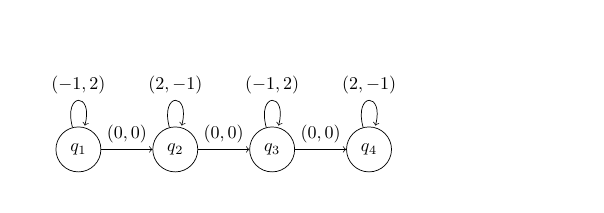
\begin{tikzpicture}[scale=0.25]
\usetikzlibrary{automata, positioning}
\scalebox{0.65}{
\node[state] (q1) {$q_1$};
\node[state, right=of q1] (q2) {$q_2$};
\node[state, right=of q2] (q3) {$q_3$};
\node[state, right=of q3] (q4) {$q_4$};

\path[->] (q1) edge [loop above] node[above] {$(-1,2)$} (q1) edge node[above] {$(0,0)$} (q2); 
\path[->] (q2) edge [loop above] node[above] {$(2,-1)$} (q2) edge node[above] {$(0,0)$} (q3);
\path[->] (q3) edge [loop above] node[above] {$(-1,2)$} (q3) edge node[above] {$(0,0)$} (q4);
\path[->] (q4) edge [loop above] node[above] {$(2,-1)$} (q4);
}
\end{tikzpicture}
\end{minipage}
\begin{minipage}{0.32\textwidth}
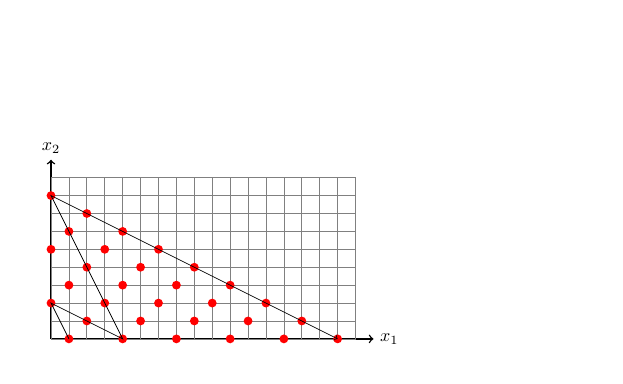
\begin{tikzpicture}[scale=0.35]
\scalebox{0.65}{
\draw[->, thick] (0, 0) -- (18, 0) node[right] {$x_1$};
\draw[->, thick] (0, 0) -- (0, 10) node[above] {$x_2$};

\draw[step=1, gray, thin] (0, 0) grid (17, 9);

\foreach \x in {1,4,7,10,13,16} \fill[red] (\x,0) circle (7pt);
\foreach \x in {2,5,8,11,14} \fill[red] (\x,1) circle (7pt);
\foreach \x in {0,3,6,9,12} \fill[red] (\x,2) circle (7pt);
\foreach \x in {1,4,7,10} \fill[red] (\x,3) circle (7pt);
\foreach \x in {2,5,8} \fill[red] (\x,4) circle (7pt);
\foreach \x in {0,3,6} \fill[red] (\x,5) circle (7pt);
\foreach \x in {1,4} \fill[red] (\x,6) circle (7pt);
\foreach \x in {2} \fill[red] (\x,7) circle (7pt);
\foreach \x in {0} \fill[red] (\x,8) circle (7pt);

\draw[->] (1,0) -- (0,2) -- (2,1) -- (4,0) -- (3,2) -- (2,4) -- (1,6) -- (0,8) -- (2,7) -- (4,6) -- (6,5) -- (8,4) -- (10,3) -- (12,2) -- (14,1) -- (16,0);
}
\end{tikzpicture}
\end{minipage}
\begin{minipage}{0.32\textwidth}
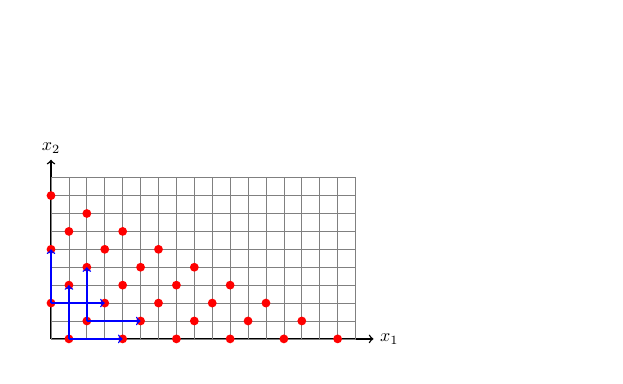
\begin{tikzpicture}[scale=0.35]
\scalebox{0.65}{
\draw[->, thick] (0, 0) -- (18, 0) node[right] {$x_1$};
\draw[->, thick] (0, 0) -- (0, 10) node[above] {$x_2$};

\draw[step=1, gray, thin] (0, 0) grid (17, 9);

\foreach \x in {1,4,7,10,13,16} \fill[red] (\x,0) circle (7pt);
\foreach \x in {2,5,8,11,14} \fill[red] (\x,1) circle (7pt);
\foreach \x in {0,3,6,9,12} \fill[red] (\x,2) circle (7pt);
\foreach \x in {1,4,7,10} \fill[red] (\x,3) circle (7pt);
\foreach \x in {2,5,8} \fill[red] (\x,4) circle (7pt);
\foreach \x in {0,3,6} \fill[red] (\x,5) circle (7pt);
\foreach \x in {1,4} \fill[red] (\x,6) circle (7pt);
\foreach \x in {2} \fill[red] (\x,7) circle (7pt);
\foreach \x in {0} \fill[red] (\x,8) circle (7pt);

\draw[->,blue,thick] (1,0) -- (4,0);
\draw[->,blue,thick] (1,0) -- (1,3);

\draw[->,blue,thick] (2,1) -- (5,1);
\draw[->,blue,thick] (2,1) -- (2,4);

\draw[->,blue,thick] (0,2) -- (3,2);
\draw[->,blue,thick] (0,2) -- (0,5);
}
\end{tikzpicture}
\end{minipage}
\caption{Left: 4-component \dvass $V_2$. 
Middle: the set $\reach_{q_4}(V_2, q_1(1,0))$ and a path $q_1(1,0) \tran q_4(16,0)$.
Right: bases 
%$A = \{(1,0),(2,1),(0,2)\}$ 
and periods 
%$P = \{(0,3),(3,0)\}$
 of an over-approximating semi-linear set $A+P^*$.}
\label{fig:zigzag}
\end{figure}

\begin{example}
For $k\geq 1$, let $V_k$ be a $(2k)$-component \dvass, where each component has just one state $q_i$
and one transition:
$(q_i, (-1,2), q_i)$ for odd $i$, and $(q_i, (2,-1), q_i)$ for even $i$.
Bridge transitions are $(q_i, (0,0), q_{i+1})$.
Figure~\ref{fig:zigzag} shows $V_2$ (left) and 
a path in $V_2$ from $s = q_1(1,0)$ to $t = q_4(16,0)$ together with 
the reachability set $\reach_{q_4}(V_2, s)$ (middle).
In general,
\begin{align} \label{eq:reachk}
X_k := \reach_{q_{2k}}(V_k, s) \ = \ \set{(x_1,x_2) \mid x_1+2x_2 \leq 4^k, \  x_1+2x_2 \equiv 1 \!\! \mod 3}.
\end{align}
Even if the size of the reachability set is 
exponential in $k$, for small $(x_1, x_2)$ it is periodic and the periods are small.
The set $X_k$ can be over-approximated by $A + P^*$ for $A = \set{(1,0),(2,1),(0,2)}$ and $P = \set{(0,3),(3,0)}$
(shown on the right of Figure~\ref{fig:zigzag}), namely for every $k\geq 1$ and $B\in\N$,
the set $X_k$ is \kanapka {$8$} {$B$}. 
For illustration, consider $Y := X_k \cap ((1,0) + P^*)$.
If $(1,0) + P^{\leq B} \subseteq X_k$ then $Y$ is a $B$-approximation
of $(1,0) + P^*$ with $\norm((1,0)), \norm(P) \leq 3 \leq 8$. 
Otherwise, there is some $(v_1, v_2) \in \big((1,0) + P^{\leq B}\big)\setminus X_k$, and
then $B$ is larger than $4^k$:
\[
%8B \geq 2(1 + 3B) \geq 2(v_1 + v_2) \geq v_1 + 2 v_2 > 
4^k < v_1 + 2 v_2 \leq 2(v_1 + v_2) \leq 2(1+3B) \leq 8B.
\]
Therefore by \eqref{eq:reachk}, each $(x_1,x_2) \in Y$ satisfies 
$\norm(x_1,x_2) = x_1 + x_2 \leq x_1 + 2x_2 \leq 4^k < 8B$, and thus
$Y$, seen as a union of singletons, is a union of 
linear sets with norm of base bounded by $8B$ and empty set of periods. 
In both cases, 
$Y$ is \kanapka {$8$} {$B$}. 
%The same intuition stays behind polynomial approximability of \dvass stated in Lemma~\ref{lem:2vass-sandwich}.
\end{example}

\section{Temporal Representation Alignment}
\label{sec:approach}

When training a series of short-horizon goal-reaching and instruction-following tasks, our goal is to learn a representation space such that our policy can generalize to a new (long-horizon) task that can be viewed as a sequence of known subtasks.
We propose to structure this representation space by aligning the representations of states, goals, and language in a way that is more amenable to compositional generalization.

\paragraph{Notation.}
We take the setting of a goal- and language-conditioned MDP $\cM$ with state space $\cS$, continuous action space $\cA \subseteq (0,1)^{d_{\cA}}$, initial state distribution $p_0$, dynamics $\p(s'\mid s,a)$, discount factor $\gamma$, and language task distribution $p_{\ell}$.
A policy $\pi(a\mid s)$ maps states to a distribution over actions. We inductively define the $k$-step (action-conditioned) policy visitation distribution as:
\begin{align*}
    p^{\pi}_{1}(s_{1} \mid s_1, a_{1})
    &\triangleq p(s_1 \mid s_1, a_1),\\
    p^{\pi}_{k+1}(s_{k+1} \mid s_1, a_1)
    &\triangleq \nonumber\\*
      &\mspace{-120mu} \int_{\cA}\int_{\cS} p(s_{k+1} \mid s,a) \dd p^{\pi}_{k}(s \mid s_{1},a_1) \dd
        \pi(a \mid s)\\
    p^{\pi}_{k+t}(s_{k+t} \mid s_t,a_t)
    &\triangleq p^{\pi}(s_{k} \mid s_1, a_1) . \eqmark
        \label{eq:successor_distribution}
\end{align*}
Then, the discounted state visitation distribution can be defined as the distribution over $s^{+}$\llap, the state reached after $K\sim \operatorname{Geom}(1-\gamma)$ steps:
\begin{equation}
    p^{\pi}_{\gamma}(s^{+}  \mid  s,a) \triangleq \sum_{k=0}^{\infty} \gamma^{k} p^{\pi}_{k}(s^{+} \mid s,a).
    \label{eq:discounted_state_visitation}
\end{equation}

We assume access to a dataset of expert demonstrations $\cD = \{\tau_{i},\ell_i\}_{i=1}^{K}$, where each trajectory
\begin{equation}
    \tau_{i} = \{s_{t,i},a_{t,i}\}_{t=1}^{H} \in \cS \times \cA
    \label{eq:trajectory}
\end{equation}
is gathered by an expert policy $\expert$, and is then annotated with $p_{\ell}(\ell_{i} \mid s_{1,i}, s_{H,i})$.
Our aim is to learn a policy $\pi$ that can select actions conditioned on a new language instruction $\ell$.
As in prior work~\citep{walke2023bridgedata}, we handle the continuous action space by representing both our policy and the expert policy as an isotropic Gaussian with fixed variance; we will equivalently write $\pi(a\mid s, \varphi)$ or denote the mode as $\hat{a} = \pi(s,\varphi)$ for a task $\varphi$.

\begin{rebuttal}
    \subsection{Representations for Reaching Distant Goals}
    \label{sec:reaching_goals}

    We learn a goal-conditioned policy $\pi(a\mid s,g)$ that selects actions to reach a goal $g$ from expert demonstrations with behavioral cloning.
    Suppose we directly selected actions to imitate the expert on two trajectories in $\cD$:
    
    \begin{equation}
        \mspace{-100mu}\begin{tikzcd}[remember picture,sep=small]
            s_1 \rar & s_2 \rar  & \ldots \rar & s_{H} \rar & w      \quad \\
            w \rar   & s_1' \rar & \ldots \rar & s_{H}' \rar & g\quad
        \end{tikzcd}
        \begin{tikzpicture}[remember picture,overlay] \coordinate (a) at (\tikzcdmatrixname-1-5.north east);
            \coordinate (b) at (\tikzcdmatrixname-2-5.south east);
            \coordinate (c) at (a|-b);
            \draw[decorate,line width=1.5pt,decoration={brace,raise=3pt,amplitude=5pt}]
        (a) -- node[right=1.5em] {$\tau_{i}\in \cD$} (c); \end{tikzpicture}
        \label{eq:trajectory_diagram}
    \end{equation}
    When conditioned with the composed goal $g$, we would be unable to imitate effectively
        as the composed state-goal $(s,g)$ is jointly out of the training distribution.

    What \emph{would} work for reaching $g$ is to first condition the policy on the intermediate waypoint $w$, then upon reaching $w$, condition on the goal $g$, as the state-goal pairs $(s_{i},w)$, $(w,g)$, and $(s_{i}',g)$ are all in the training distribution.
    If we condition the policy on some intermediate waypoint distribution $p(w)$ (or sufficient statistics thereof) that captures all of these cases, we can stitch together the expert behaviors to reach the goal $g$.

    Our approach is to learn a representation space that captures this ability, so that a GCBC objective used in this space can effectively imitate the expert on the composed task.
     We begin with the goal-conditioned behavioral cloning~\citep{kaelbling1993learning}
        loss $\cL_{\textsc{bc}}^{\phi,\psi,\xi}$ conditioned with waypoints $w$.
    \begin{equation}
        \cL_{\textsc{bc}}\bigl(\{s_{i},a_{i},s_{i}^{+},g_{i}\}_{i=1}^{K}\bigr) = \sum_{{i=1}}^{K} \log \pi\bigl(a_{i} \mid s_{i},\psi(g_{i})\bigr).
        \label{eq:goal_conditioned_bc}
    \end{equation}
    Enforcing the invariance needed to stitch \cref{eq:trajectory_diagram} then reduces to aligning \mbox{$\psi(g) \leftrightarrow \psi(w).$}
    The temporal alignment objective $\phi(s)\leftrightarrow \phi(s^{+})$ accomplishes this indirectly by aligning both $\psi(w)$ and $\psi(g)$ to the shared waypoint representation $\phi(w)$:

    \csuse{color indices}
    \begin{align}
        &\cL_{\textsc{nce}}\bigl(\{s_{i},s_{i}^{+}\}_{i=1}^{K};\phi,\psi\bigr) =
        \log \biggl( {\frac{e^{\phi(s^+_{\i})^{T}\psi(s_{\i})}}{\sum_{{\j=1}}^{K}
                e^{\phi(s^+_{\i})^{T}\psi(s_{\j})}}} \biggr)  \nonumber\\*
                &\mspace{100mu} +
        \sum_{{\j=1}}^{K} \log \biggl( {\frac{e^{\phi(s^+_{\i})^{T}\psi(s_{\i})}}{\sum_{{\i=1}}^{K}
                e^{\phi(s^+_{\i})^{T}\psi(s_{\j})}}} \biggr)
        \label{eq:goal_alignment}
    \end{align}

        
\end{rebuttal}
\subsection{Interfacing with Language Instructions}
\label{sec:language_instructions}

To extend the representations from \cref{sec:reaching_goals} to compositional instruction following with language tasks, we need some way to ground language into the $\psi$ (future state)
representation space.
We use a similar approach to GRIF~\citep{myers2023goal}, which uses an additional CLIP-style \citep{radford2021learning} contrastive alignment loss with an additional pretrained language encoder $\xi$:
\csuse{no color indices}
\begin{align}
    &\cL_{\textsc{nce}}\bigl(\{g_{i},\ell_{i}\}_{i=1}^{K};\psi,\xi\bigr)
    = \sum_{{i=1}}^{K} \log \biggl( {\frac{e^{\psi(g_{\i})^{T}\xi(\ell_{\i})}}{\sum_{{\j=1}}^{K}
            e^{\psi(g_{\i})^{T}\xi(\ell_{\j})}}} \biggr)  \nonumber\\*
            &\mspace{100mu} +
    \sum_{{\j=1}}^{K} \log \biggl( {\frac{e^{\psi(g_{\i})^{T}\xi(\ell_{\i})}}{\sum_{{\i=1}}^{K}
            e^{\psi(g_{\i})^{T}\xi(\ell_{\j})}}} \biggr)
    \label{eq:task_alignment}
\end{align}

\subsection{Temporal Alignment}
\label{sec:temporal_alignment}

Putting together the objectives from \cref{sec:reaching_goals,sec:language_instructions} yields the Temporal Representation Alignment (\Method) approach.
\Method{} structures the representation space of goals and language instructions to better enable compositional generalization.
We learn encoders $\phi, \psi ,$ and $\xi$ to map states, goals, and language instructions to a shared representation space.

\csuse{color indices}
\begin{align}
    \cL_{\textsc{nce}} \label{eq:NCE}
    &(\{x_{i}, y_{i}\}_{i=1}^{K};f,h) =
        \sum_{{\i=1}}^{K} \log \biggl( {\frac{e^{f(y_{\i})^{T}h(x_{\i})}}{\sum_{{\j=1}}^{K}
        e^{f(y_{\i})^{T}h(x_{\j})}}} \biggr) \nonumber\\*
      &\mspace{100mu} +
        \sum_{{\j=1}}^{K} \log \biggl( {\frac{e^{f(y_{\i})^{T}h(x_{\i})}}{\sum_{{\i=1}}^{K}
        e^{f(y_{\i})^{T}h(x_{\j})}}} \biggr) \\
    \cL_{\textsc{bc}} \label{eq:BC}
    &\bigl(\{s_{i},a_{i},s^{+}_{i},\ell_{i}\}_{i=1}^{K};\pi,\psi,\xi\bigr) = \nonumber\\*
      &\mspace{-10mu} \sum_{{i=1}}^{K} \log
        \pi\bigl(a_{i} \mid s_{i},\xi(\ell_{i})\bigr) + \log \pi\bigl(a_{i} \mid
        s_{i},\psi(s^{+}_{i})\bigr) \\
    \cL_{\textsc{tra}}
    &\label{eq:TRA} \bigl( \{s_{i},a_{i},s_{i}^{+},g_{i},\ell_{i}\}_{i=1}^{K}; \pi,\phi,\psi,\xi\bigr)
        \\
    &= \underbrace{\cL_{\textsc{bc}}\bigl(\{s_{i},a_{i},s_{i}^{+},\ell_{i}\}_{i=1}^{K};\pi,\psi,\xi\bigr)}_{\text{behavioral
    cloning}} \nonumber\\*
    &+
        \underbrace{\cL_{\textsc{nce}}\bigl(\{s_{i},s_{i}^{+}\}_{i=1}^{K};\phi,\psi\bigr)}_{\text{temporal alignment}}
        + \underbrace{\cL_{\textsc{nce}}\bigl(\{g_{i},\ell_{i}\}_{i=1}^{K};\psi,\xi\bigr)}_{\text{task alignment}} \nonumber
\end{align}Note that the NCE alignment loss uses a CLIP-style symmetric contrastive objective~\citep{radford2021learning,eysenbach2024inference} \-- we highlight the indices in the NCE alignment loss~\eqref{eq:NCE} for clarity.

Our overall objective is to minimize \cref{eq:TRA} across states, actions, future states, goals, and language tasks within the training data:
\begin{align}
    &\min_{\pi,\phi,\psi,\xi} \mathbb{E}_{\substack{(s_{1,i},a_{1,i},\ldots,s_{H,i},a_{H,i},\ell) \sim \mathcal{D} \\
    i\sim\operatorname{Unif}(1\ldots H) \\
    k\sim\operatorname{Geom}(1-\gamma)}} \\*
    &\mspace{10mu}
    \Bigl[\cL_{\text{TRA}}\bigl(\{s_{t,i},a_{t,i},s_{\min(t+k,H),i},s_{H,i},\ell\}_{i=1}^{K};\pi,\phi,\psi,\xi\bigr)\Bigr].
    \label{eq:overall_objective}
\end{align}

\begin{algorithm}
    \caption{Temporal Representation Alignment}
    \label{alg:tra}
    \begin{algorithmic}[1]
        \State \textbf{input:} dataset $\mathcal{D} = (\{s_{t,i},a_{t,i}\}_{t=1}^{H},\ell_i)_{i=1}^N$
        \State initialize networks $\Theta \triangleq (\pi,\phi,\psi,\xi)$
        \While{training}
        \State sample batch $\bigl\{(s_{t,i},a_{t,i},s_{t+k,i},\ell_i)\bigr\}_{i=1}^K\sim\mathcal{D}$ \\
        \hspace*{2ex} for $k\sim\operatorname{Geom}(1-\gamma)$
        \State $\Theta \gets \Theta - \alpha \nabla_{\Theta} \cL_{\text{TRA}}\bigl(\{s_{t,i},a_{t,i},s_{t+k,i},\ell_i\}_{i=1}^K; \Theta\bigr)$
        \EndWhile
        \smallskip
        \State \textbf{output:} \parbox[t]{\linewidth}{language-conditioned policy $\pi(a_{t} | s_{t}, \xi(\ell))$ \\
            goal-conditioned policy $\pi(a_{t} | s_{t}, \psi(g))$
        }
    \end{algorithmic}
\end{algorithm}

\subsection{Implementation}
\label{sec:implementation}

A summary of our approach is shown in \cref{alg:tra}.
In essence, TRA learns three encoders: $\phi$, which encodes states, $\psi$ which encodes future goals, and $\xi$ which encodes language instructions.
Contrastive losses are used to align state representations $\phi(s_{t})$ with future goal representations $\psi(s_{t+k})$, which are in turn aligned with equivalent language task specifications $\xi(\ell)$ when available.
We then learn a behavior cloning policy $\pi$ that can be conditioned on either the goal or language instruction through the representation $\psi(g)$ or $\xi(\ell)$, respectively.

\begin{rebuttal}
    \subsection{Temporal Alignment and Compositionality}
    \label{sec:compositionality}

    We will formalize the intuition from \cref{sec:reaching_goals} that \Method{} enables compositional generalization by considering the error on a ``compositional'' version of $\cD,$ denoted $\cD^{*}$.
    Using the notation from \cref{eq:trajectory}, we can say $\cD$ is distributed according to:
    \begin{align}
        &\cD \triangleq \cD^{H} \sim \prod_{i=1}^{K} p_0(s_{1,i}) p_{\ell}(\ell_{i} \mid s_{1,i}, s_{H,i})
            \nonumber\\*
          &\mspace{60mu} \prod_{t=1}^{H} \expert(a_{t,i} \mid s_{t,i}) \p(s_{t+1,i} \mid s_{t,i}, a_{t,i}) ,
            \label{eq:dataset_distribution}
    \end{align}
    or equivalently
    \begin{align}
            &\cD^{H} \sim \prod_{i=1}^{K} p_0(s_{1,i}) p_{\ell}(\ell_{i} \mid s_{1,i}, s_{H,i}) \nonumber\\*
            &\mspace{60mu} \prod_{t=1}^{H}
            e^{\sigma^2\|\expert(s_{t,i}) - a_{t,i}\|^2}\p(s_{t+1,i} \mid s_{t,i}, a_{t,i}) ,
            \label{eq:dataset_distribution_2}
    \end{align}
    by the isotropic Gaussian assumption.
    We will define $\cD^{*} \triangleq \cD^{H'}$ to be a longer-horizon version of $\cD$ extending the behaviors gathered under $\expert$ across a horizon $\alpha H \ge H' \ge H$ that additionally satisfies a ``time-isotropy'' property: the marginal distribution of the states is uniform across the horizon, i.e., $p_0(s_{1,i}) = p_0(s_{t,i})$ for all $t \in \{1\ldots H'\}$.

    We will relate the in-distribution imitation error $\textsc{Err}(\bullet; \cD)$ to the compositional out-of-distribution imitation error $\textsc{Err}(\bullet;\cD^{*})$.
    We define
    \begin{align}
        \textsc{Err}(\hat{\pi}; \tilde{\cD})
        &= \E_{\tilde{\cD}}\Bigl[\frac{1}{H}\sum_{t=1}^{H} \mathbb{E}_{\hat{\pi}}\left[\|\tilde{a}_{t,i} -
        \hat{\pi}(\tilde{s}_{t,i}, \tilde{s}_{H, i})\|^{2}/d_{\cA}\right]\Bigr] \nonumber\\
        &\quad \text{for} \quad \{\tilde{s}_{t,i},\tilde{a}_{t,i},\tilde{\ell}_{i}\}_{t=1}^{H} \sim
            \tilde{\cD}.
            \label{eq:imitation_error}
    \end{align}
    On the training dataset this is equivalent to the expected behavioral cloning loss from \cref{eq:BC}.

                            
    \begin{assumption}
        \label{asm:policy_factorization}
        The policy factorizes through inferred waypoints as:
\begin{align}
    &\textrm{goals: }\pi(a \mid s, g)
        = \nonumber\\*
      &\mspace{50mu} \int \pi(a\mid s, w) \p(s_{t}=w \mid s_{t+k}=g) \dd{w}
        \label{eq:goal-conditioned} \\
    &\textrm{language: } \pi(a \mid s, \ell)
        = \int \pi(a\mid s, w) \nonumber\\*
      &\mspace{20mu} \p(s_{t}=w \mid s_{t+k}=g) \p(s_{t+k}=g \mid \ell) \dd{w} \dd{g} ,
        \label{eq:language-conditioned}
        \end{align}
        where denote by $\pi(s,g)$ the MLE estimate of the action $a$.

    \end{assumption}

    \makerestatable
    \begin{theorem}
        \label{thm:compositionality}
        Suppose $\cD$ is distributed according to \cref{eq:dataset_distribution} and $\cD^{*}$ is distributed according to \cref{eq:dataset_distribution}.
        When $\gamma > 1-1/H$ and $\alpha > 1$, for optimal features $\phi$ and $\psi$ under \cref{eq:overall_objective}, we have
        \begin{gather}
            \textsc{Err}(\pi; \cD^{*}) \le \textsc{Err}(\pi; \cD) +  \frac{\alpha -1}{2 \alpha }+\Bigl(\frac{ \alpha - 2 }{2\alpha}\Bigr) \1 \{\alpha >2\}  .
            \label{eq:compositionality}
        \end{gather}
    \end{theorem}

    We can also define a notion of the language-conditioned compositional generalization error:
    \begin{equation*}
        \errl(\pi; \cD^{*}) \triangleq \E_{\cD^{*}}\Bigl[\frac{1}{H}\sum_{t=1}^{H}
            \mathbb{E}_{\pi}\bigl[\|\tilde{a}_{t,i} - \pi(\tilde{s}_{t,i}, \tilde{\ell}_{i})\|^{2}\bigr]\Bigr].
            \label{eq:language_error}
    \end{equation*}

    \makerestatable
    \begin{corollary}
        \label{thm:language}
        Under the same conditions as \cref{thm:compositionality},
        \begin{equation*}
            \errl(\pi; \cD^{*}) \le \errl(\pi; \cD) +  \frac{\alpha -1}{2 \alpha }+\Bigl(\frac{ \alpha - 2 }{2\alpha}\Bigr) \1 \{\alpha >2\}  .
            \label{eq:compositionality_language}
        \end{equation*}

    \end{corollary}

    The proofs as well as a visualization of the bound are in \cref{app:compositionality}. Policy implementation details can be found in \cref{app:tra_impl}

    
                
        
    \end{rebuttal}


\definecolor{darkgreen}{rgb}{0.0, 0.5, 0.0}
\definecolor{violet}{rgb}{0.56, 0.0, 1.0}
\section{Evaluation}
We apply our methodology to derive counterfactual policies for various MDPs, addressing three main research questions: (1) how does our policy's performance compare to the Gumbel-max SCM approach; (2) how do the counterfactual stability and monotonicity assumptions impact the probability bounds; and (3) how fast is our approach compared with the Gumbel-max SCM method?

\begin{figure*}
    \centering
    %
    \resizebox{0.6\textwidth}{!}{
        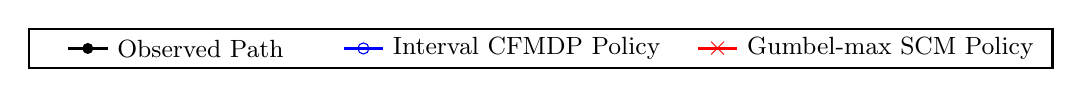
\begin{tikzpicture}[scale=1.0, every node/.style={scale=1.0}]
            \draw[thick, black] (-3, -0.25) rectangle (10, 0.25);
            %
            \draw[black, line width=1pt] (-2.5, 0.0) -- (-2,0.0);
            \fill[black] (-2.25,0.0) circle (2pt); %
            \node[right] at (-2,0.0) {\small Observed Path};
            
            %
            \draw[blue, line width=1pt] (1.0,0.0) -- (1.5,0.0);
            \node[draw=blue, circle, minimum size=4pt, inner sep=0pt] at (1.25,0.0) {}; %
            \node[right] at (1.5,0.0) {\small Interval CFMDP Policy};
            
            %
            \draw[red, line width=1pt] (5.5,0) -- (6,0);
            \node[red] at (5.75,0) {$\boldsymbol{\times}$}; %
            \node[right] at (6,0) {\small Gumbel-max SCM Policy};
        \end{tikzpicture}
    }\\
    %
    \subfigure[\footnotesize Lowest cumulative reward: Interval CFMDP ($312$), Gumbel-max SCM ($312$)]{%
        \resizebox{0.76\columnwidth}{!}{
             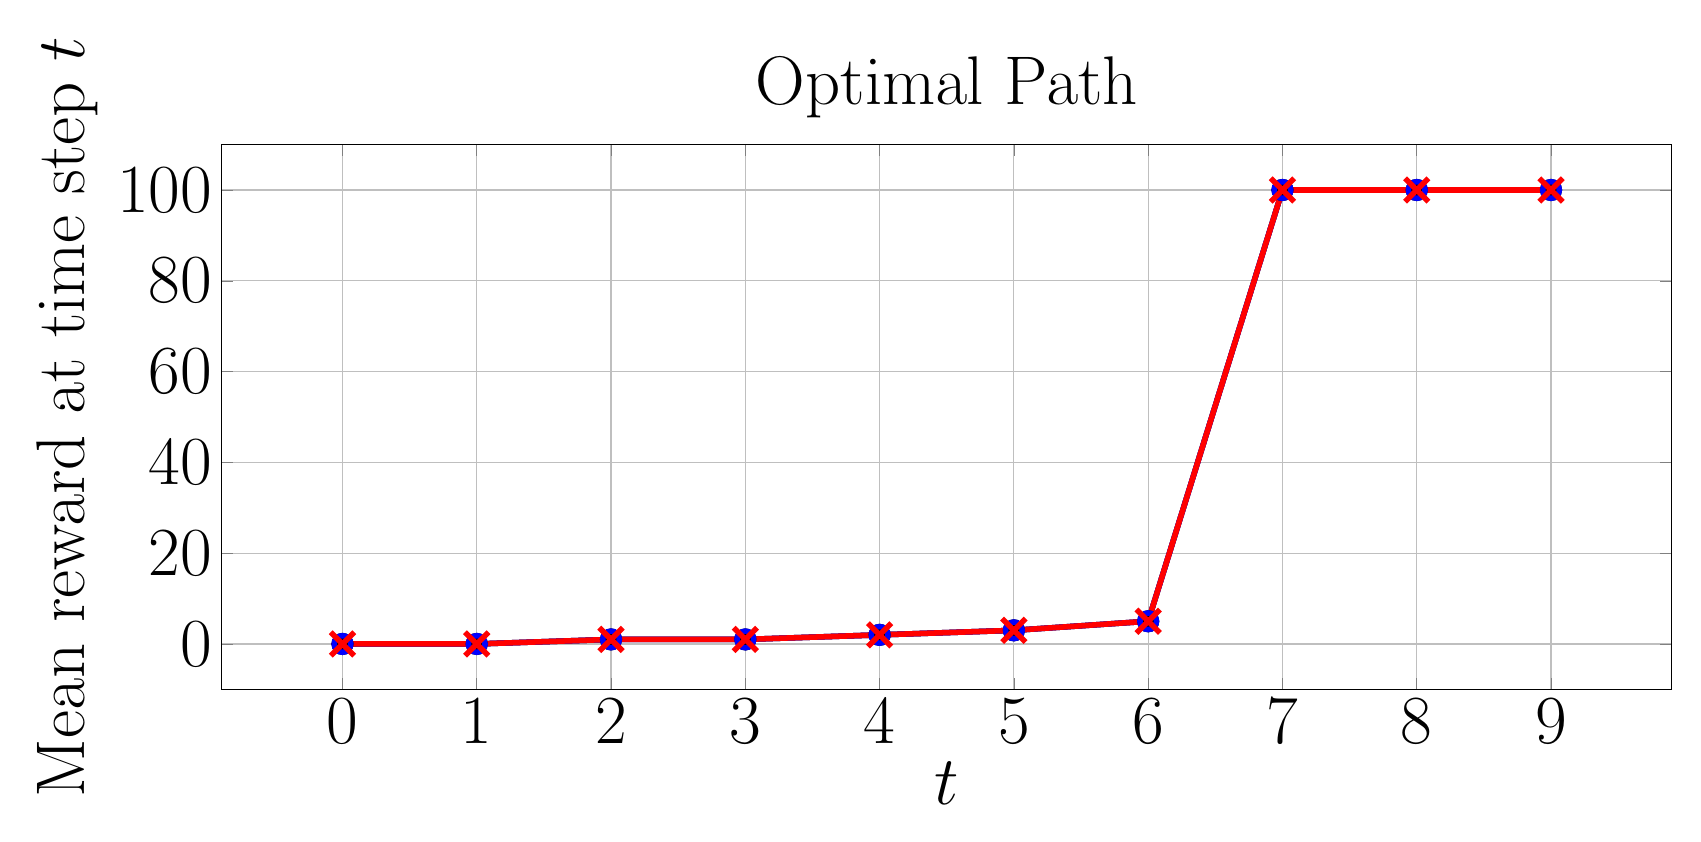
\begin{tikzpicture}
                \begin{axis}[
                    xlabel={$t$},
                    ylabel={Mean reward at time step $t$},
                    title={Optimal Path},
                    grid=both,
                    width=20cm, height=8.5cm,
                    every axis/.style={font=\Huge},
                    %
                ]
                \addplot[
                    color=black, %
                    mark=*, %
                    line width=2pt,
                    mark size=3pt,
                    error bars/.cd,
                    y dir=both, %
                    y explicit, %
                    error bar style={line width=1pt,solid},
                    error mark options={line width=1pt,mark size=4pt,rotate=90}
                ]
                coordinates {
                    (0, 0.0)  +- (0, 0.0)
                    (1, 0.0)  +- (0, 0.0) 
                    (2, 1.0)  +- (0, 0.0) 
                    (3, 1.0)  +- (0, 0.0)
                    (4, 2.0)  +- (0, 0.0)
                    (5, 3.0) +- (0, 0.0)
                    (6, 5.0) +- (0, 0.0)
                    (7, 100.0) +- (0, 0.0)
                    (8, 100.0) +- (0, 0.0)
                    (9, 100.0) +- (0, 0.0)
                };
                %
                \addplot[
                    color=blue, %
                    mark=o, %
                    line width=2pt,
                    mark size=3pt,
                    error bars/.cd,
                    y dir=both, %
                    y explicit, %
                    error bar style={line width=1pt,solid},
                    error mark options={line width=1pt,mark size=4pt,rotate=90}
                ]
                 coordinates {
                    (0, 0.0)  +- (0, 0.0)
                    (1, 0.0)  +- (0, 0.0) 
                    (2, 1.0)  +- (0, 0.0) 
                    (3, 1.0)  +- (0, 0.0)
                    (4, 2.0)  +- (0, 0.0)
                    (5, 3.0) +- (0, 0.0)
                    (6, 5.0) +- (0, 0.0)
                    (7, 100.0) +- (0, 0.0)
                    (8, 100.0) +- (0, 0.0)
                    (9, 100.0) +- (0, 0.0)
                };
                %
                \addplot[
                    color=red, %
                    mark=x, %
                    line width=2pt,
                    mark size=6pt,
                    error bars/.cd,
                    y dir=both, %
                    y explicit, %
                    error bar style={line width=1pt,solid},
                    error mark options={line width=1pt,mark size=4pt,rotate=90}
                ]
                coordinates {
                    (0, 0.0)  +- (0, 0.0)
                    (1, 0.0)  +- (0, 0.0) 
                    (2, 1.0)  +- (0, 0.0) 
                    (3, 1.0)  +- (0, 0.0)
                    (4, 2.0)  +- (0, 0.0)
                    (5, 3.0) +- (0, 0.0)
                    (6, 5.0) +- (0, 0.0)
                    (7, 100.0) +- (0, 0.0)
                    (8, 100.0) +- (0, 0.0)
                    (9, 100.0) +- (0, 0.0)
                };
                \end{axis}
            \end{tikzpicture}
         }
    }
    \hspace{1cm}
    \subfigure[\footnotesize Lowest cumulative reward: Interval CFMDP ($19$), Gumbel-max SCM ($-88$)]{%
         \resizebox{0.76\columnwidth}{!}{
            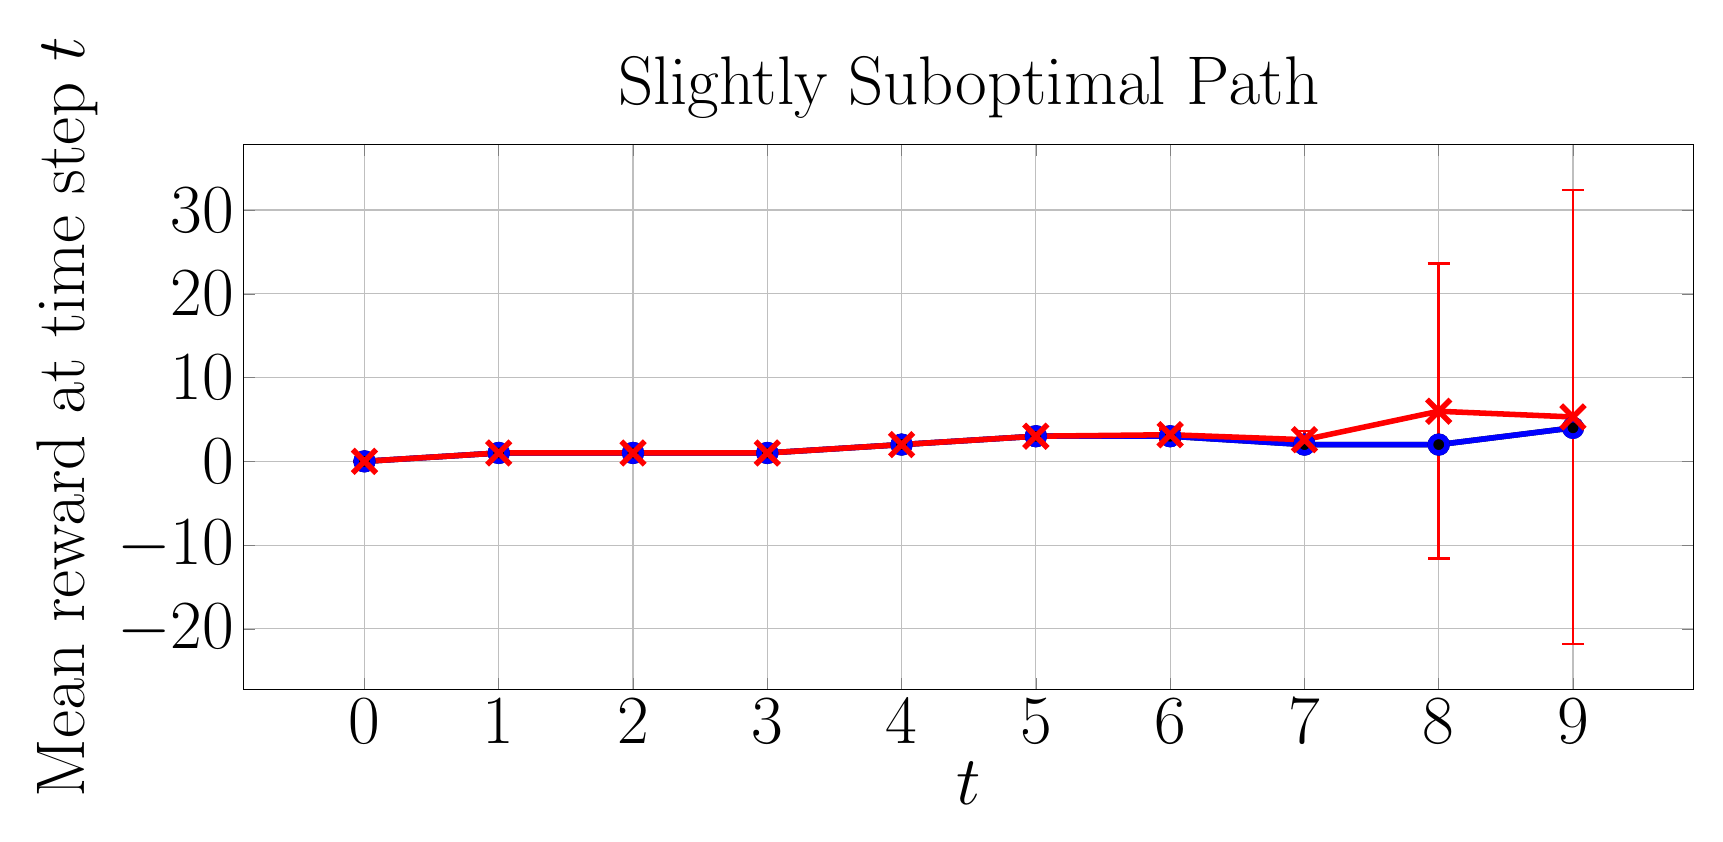
\begin{tikzpicture}
                \begin{axis}[
                    xlabel={$t$},
                    ylabel={Mean reward at time step $t$},
                    title={Slightly Suboptimal Path},
                    grid=both,
                    width=20cm, height=8.5cm,
                    every axis/.style={font=\Huge},
                    %
                ]
                \addplot[
                    color=black, %
                    mark=*, %
                    line width=2pt,
                    mark size=3pt,
                    error bars/.cd,
                    y dir=both, %
                    y explicit, %
                    error bar style={line width=1pt,solid},
                    error mark options={line width=1pt,mark size=4pt,rotate=90}
                ]
              coordinates {
                    (0, 0.0)  +- (0, 0.0)
                    (1, 1.0)  +- (0, 0.0) 
                    (2, 1.0)  +- (0, 0.0) 
                    (3, 1.0)  +- (0, 0.0)
                    (4, 2.0)  +- (0, 0.0)
                    (5, 3.0) +- (0, 0.0)
                    (6, 3.0) +- (0, 0.0)
                    (7, 2.0) +- (0, 0.0)
                    (8, 2.0) +- (0, 0.0)
                    (9, 4.0) +- (0, 0.0)
                };
                %
                \addplot[
                    color=blue, %
                    mark=o, %
                    line width=2pt,
                    mark size=3pt,
                    error bars/.cd,
                    y dir=both, %
                    y explicit, %
                    error bar style={line width=1pt,solid},
                    error mark options={line width=1pt,mark size=4pt,rotate=90}
                ]
              coordinates {
                    (0, 0.0)  +- (0, 0.0)
                    (1, 1.0)  +- (0, 0.0) 
                    (2, 1.0)  +- (0, 0.0) 
                    (3, 1.0)  +- (0, 0.0)
                    (4, 2.0)  +- (0, 0.0)
                    (5, 3.0) +- (0, 0.0)
                    (6, 3.0) +- (0, 0.0)
                    (7, 2.0) +- (0, 0.0)
                    (8, 2.0) +- (0, 0.0)
                    (9, 4.0) +- (0, 0.0)
                };
                %
                \addplot[
                    color=red, %
                    mark=x, %
                    line width=2pt,
                    mark size=6pt,
                    error bars/.cd,
                    y dir=both, %
                    y explicit, %
                    error bar style={line width=1pt,solid},
                    error mark options={line width=1pt,mark size=4pt,rotate=90}
                ]
                coordinates {
                    (0, 0.0)  +- (0, 0.0)
                    (1, 1.0)  +- (0, 0.0) 
                    (2, 1.0)  +- (0, 0.0) 
                    (3, 1.0)  +- (0, 0.0)
                    (4, 2.0)  += (0, 0.0)
                    (5, 3.0)  += (0, 0.0)
                    (6, 3.17847) += (0, 0.62606746) -= (0, 0.62606746)
                    (7, 2.5832885) += (0, 1.04598233) -= (0, 1.04598233)
                    (8, 5.978909) += (0, 17.60137623) -= (0, 17.60137623)
                    (9, 5.297059) += (0, 27.09227512) -= (0, 27.09227512)
                };
                \end{axis}
            \end{tikzpicture}
         }
    }\\[-1.5pt]
    \subfigure[\footnotesize Lowest cumulative reward: Interval CFMDP ($14$), Gumbel-max SCM ($-598$)]{%
         \resizebox{0.76\columnwidth}{!}{
             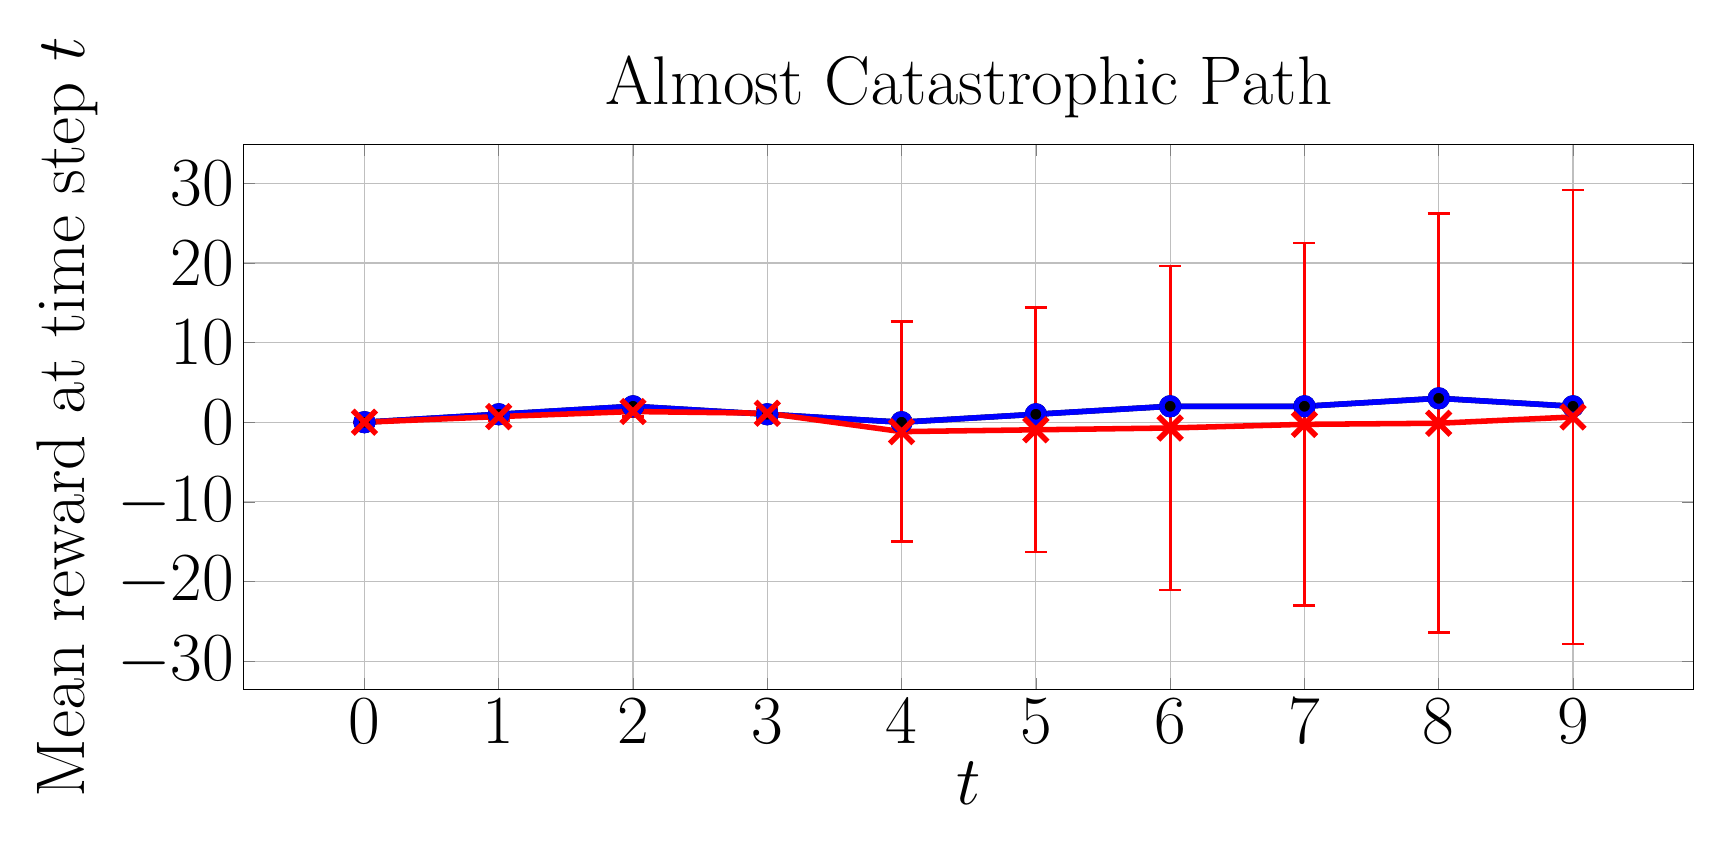
\begin{tikzpicture}
                \begin{axis}[
                    xlabel={$t$},
                    ylabel={Mean reward at time step $t$},
                    title={Almost Catastrophic Path},
                    grid=both,
                    width=20cm, height=8.5cm,
                    every axis/.style={font=\Huge},
                    %
                ]
                \addplot[
                    color=black, %
                    mark=*, %
                    line width=2pt,
                    mark size=3pt,
                    error bars/.cd,
                    y dir=both, %
                    y explicit, %
                    error bar style={line width=1pt,solid},
                    error mark options={line width=1pt,mark size=4pt,rotate=90}
                ]
                coordinates {
                    (0, 0.0)  +- (0, 0.0)
                    (1, 1.0)  +- (0, 0.0) 
                    (2, 2.0)  +- (0, 0.0) 
                    (3, 1.0)  +- (0, 0.0)
                    (4, 0.0)  +- (0, 0.0)
                    (5, 1.0) +- (0, 0.0)
                    (6, 2.0) +- (0, 0.0)
                    (7, 2.0) +- (0, 0.0)
                    (8, 3.0) +- (0, 0.0)
                    (9, 2.0) +- (0, 0.0)
                };
                %
                \addplot[
                    color=blue, %
                    mark=o, %
                    line width=2pt,
                    mark size=3pt,
                    error bars/.cd,
                    y dir=both, %
                    y explicit, %
                    error bar style={line width=1pt,solid},
                    error mark options={line width=1pt,mark size=4pt,rotate=90}
                ]
                coordinates {
                    (0, 0.0)  +- (0, 0.0)
                    (1, 1.0)  +- (0, 0.0) 
                    (2, 2.0)  +- (0, 0.0) 
                    (3, 1.0)  +- (0, 0.0)
                    (4, 0.0)  +- (0, 0.0)
                    (5, 1.0) +- (0, 0.0)
                    (6, 2.0) +- (0, 0.0)
                    (7, 2.0) +- (0, 0.0)
                    (8, 3.0) +- (0, 0.0)
                    (9, 2.0) +- (0, 0.0)
                };
                %
                \addplot[
                    color=red, %
                    mark=x, %
                    line width=2pt,
                    mark size=6pt,
                    error bars/.cd,
                    y dir=both, %
                    y explicit, %
                    error bar style={line width=1pt,solid},
                    error mark options={line width=1pt,mark size=4pt,rotate=90}
                ]
                coordinates {
                    (0, 0.0)  +- (0, 0.0)
                    (1, 0.7065655)  +- (0, 0.4553358) 
                    (2, 1.341673)  +- (0, 0.67091621) 
                    (3, 1.122926)  +- (0, 0.61281824)
                    (4, -1.1821935)  +- (0, 13.82444042)
                    (5, -0.952399)  +- (0, 15.35195457)
                    (6, -0.72672) +- (0, 20.33508414)
                    (7, -0.268983) +- (0, 22.77861454)
                    (8, -0.1310835) +- (0, 26.31013314)
                    (9, 0.65806) +- (0, 28.50670214)
                };
                %
            %
            %
            %
            %
            %
            %
            %
            %
            %
            %
            %
            %
            %
            %
            %
            %
            %
            %
                \end{axis}
            \end{tikzpicture}
         }
    }
    \hspace{1cm}
    \subfigure[\footnotesize Lowest cumulative reward: Interval CFMDP ($-698$), Gumbel-max SCM ($-698$)]{%
         \resizebox{0.76\columnwidth}{!}{
            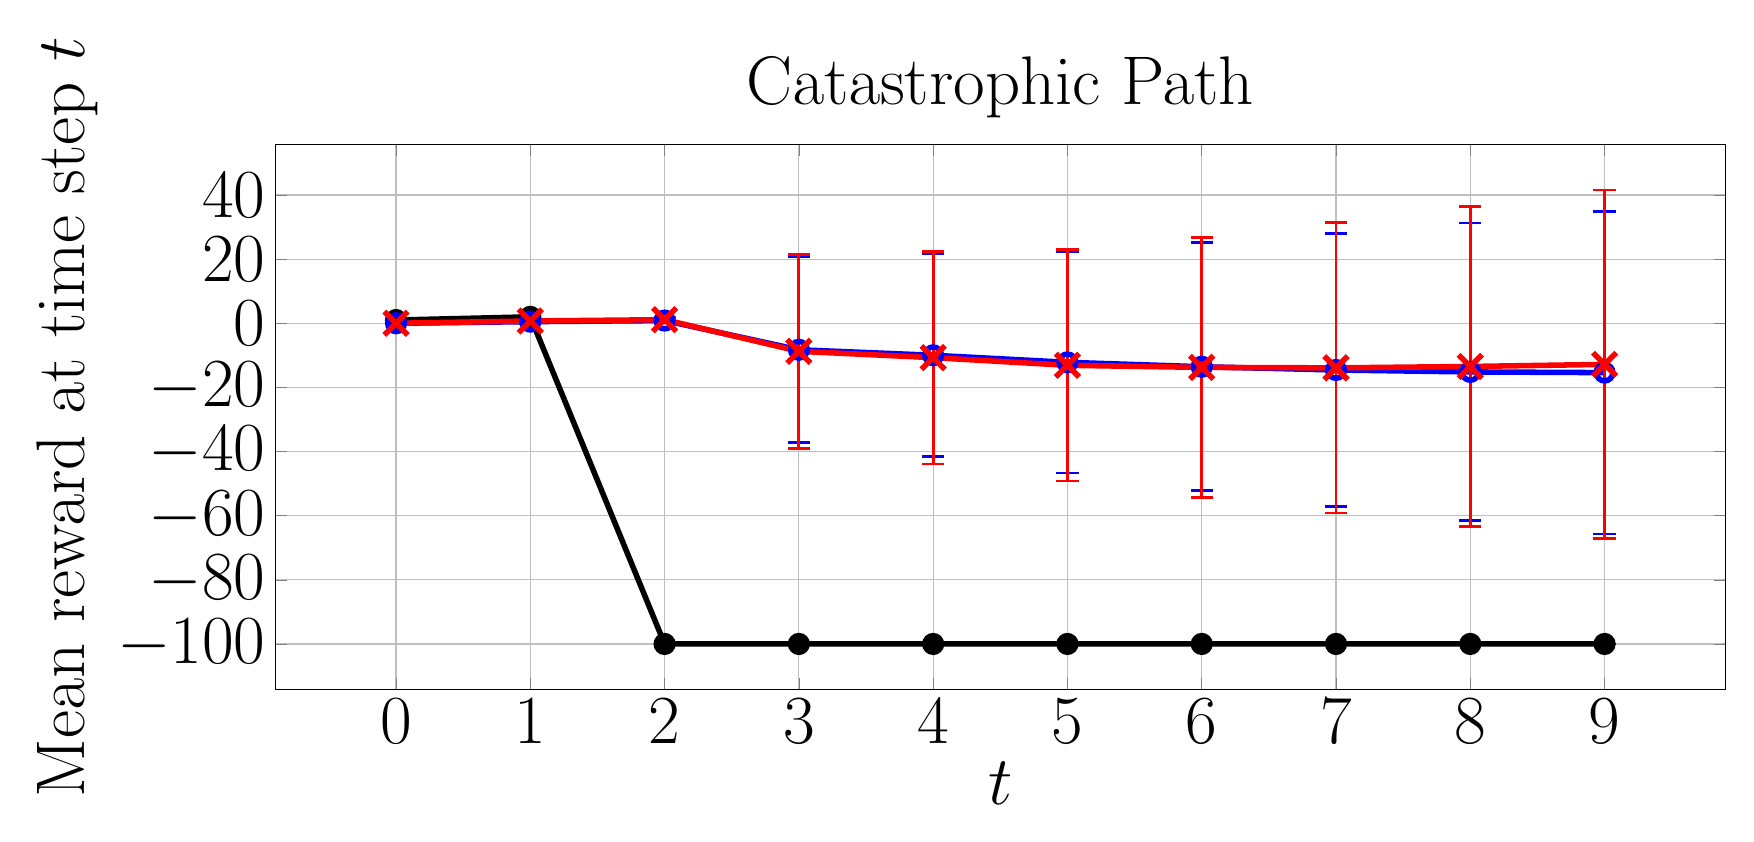
\begin{tikzpicture}
                \begin{axis}[
                    xlabel={$t$},
                    ylabel={Mean reward at time step $t$},
                    title={Catastrophic Path},
                    grid=both,
                    width=20cm, height=8.5cm,
                    every axis/.style={font=\Huge},
                    %
                ]
                \addplot[
                    color=black, %
                    mark=*, %
                    line width=2pt,
                    mark size=3pt,
                    error bars/.cd,
                    y dir=both, %
                    y explicit, %
                    error bar style={line width=1pt,solid},
                    error mark options={line width=1pt,mark size=4pt,rotate=90}
                ]
                coordinates {
                    (0, 1.0)  +- (0, 0.0)
                    (1, 2.0)  +- (0, 0.0) 
                    (2, -100.0)  +- (0, 0.0) 
                    (3, -100.0)  +- (0, 0.0)
                    (4, -100.0)  +- (0, 0.0)
                    (5, -100.0) +- (0, 0.0)
                    (6, -100.0) +- (0, 0.0)
                    (7, -100.0) +- (0, 0.0)
                    (8, -100.0) +- (0, 0.0)
                    (9, -100.0) +- (0, 0.0)
                };
                %
                \addplot[
                    color=blue, %
                    mark=o, %
                    line width=2pt,
                    mark size=3pt,
                    error bars/.cd,
                    y dir=both, %
                    y explicit, %
                    error bar style={line width=1pt,solid},
                    error mark options={line width=1pt,mark size=4pt,rotate=90}
                ]
                coordinates {
                    (0, 0.0)  +- (0, 0.0)
                    (1, 0.504814)  +- (0, 0.49997682) 
                    (2, 0.8439835)  +- (0, 0.76831917) 
                    (3, -8.2709165)  +- (0, 28.93656754)
                    (4, -9.981082)  +- (0, 31.66825363)
                    (5, -12.1776325) +- (0, 34.53463233)
                    (6, -13.556076) +- (0, 38.62845372)
                    (7, -14.574418) +- (0, 42.49603359)
                    (8, -15.1757075) +- (0, 46.41913968)
                    (9, -15.3900395) +- (0, 50.33563368)
                };
                %
                \addplot[
                    color=red, %
                    mark=x, %
                    line width=2pt,
                    mark size=6pt,
                    error bars/.cd,
                    y dir=both, %
                    y explicit, %
                    error bar style={line width=1pt,solid},
                    error mark options={line width=1pt,mark size=4pt,rotate=90}
                ]
                coordinates {
                    (0, 0.0)  +- (0, 0.0)
                    (1, 0.701873)  +- (0, 0.45743556) 
                    (2, 1.1227805)  +- (0, 0.73433129) 
                    (3, -8.7503255)  +- (0, 30.30257976)
                    (4, -10.722092)  +- (0, 33.17618589)
                    (5, -13.10721)  +- (0, 36.0648089)
                    (6, -13.7631645) +- (0, 40.56553451)
                    (7, -13.909043) +- (0, 45.23829402)
                    (8, -13.472517) +- (0, 49.96270296)
                    (9, -12.8278835) +- (0, 54.38618735)
                };
                %
            %
            %
            %
            %
            %
            %
            %
            %
            %
            %
            %
            %
            %
            %
            %
            %
            %
            %
                \end{axis}
            \end{tikzpicture}
         }
    }
    \caption{Average instant reward of CF paths induced by policies on GridWorld $p=0.4$.}
    \label{fig: reward p=0.4}
\end{figure*}

\subsection{Experimental Setup}
To compare policy performance, we measure the average rewards of counterfactual paths induced by our policy and the Gumbel-max policy by uniformly sampling $200$ counterfactual MDPs from the ICFMDP and generating $10,000$ counterfactual paths over each sampled CFMDP. \jl{Since the interval CFMDP depends on the observed path, we select $4$  paths of varying optimality to evaluate how the observed path impacts the performance of both policies: an optimal path, a slightly suboptimal path that could reach the optimal reward with a few changes, a catastrophic path that enters a catastrophic, terminal state with low reward, and an almost catastrophic path that was close to entering a catastrophic state.} When measuring the average probability bound widths and execution time needed to generate the ICFMDPs, we averaged over $20$ randomly generated observed paths
\footnote{Further training details are provided in Appendix \ref{app: training details}, and the code is provided at \href{https://github.com/ddv-lab/robust-cf-inference-in-MDPs}{https://github.com/ddv-lab/robust-cf-inference-in-MDPs}
%
%
.}.

\subsection{GridWorld}
\jl{The GridWorld MDP is a $4 \times 4$ grid where an agent must navigate from the top-left corner to the goal state in the bottom-right corner, avoiding a dangerous terminal state in the centre. At each time step, the agent can move up, down, left, or right, but there is a small probability (controlled by hyper-parameter $p$) of moving in an unintended direction. As the agent nears the goal, the reward for each state increases, culminating in a reward of $+100$ for reaching the goal. Entering the dangerous state results in a penalty of $-100$. We use two versions of GridWorld: a less stochastic version with $p=0.9$ (i.e., $90$\% chance of moving in the chosen direction) and a more stochastic version with $p=0.4$.}

\paragraph{GridWorld ($p=0.9$)}
When $p=0.9$, the counterfactual probability bounds are typically narrow (see Table \ref{tab:nonzero_probs} for average measurements). Consequently, as shown in Figure \ref{fig: reward p=0.9}, both policies are nearly identical and perform similarly well across the optimal, slightly suboptimal, and catastrophic paths.
%
However, for the almost catastrophic path, the interval CFMDP path is more conservative and follows the observed path more closely (as this is where the probability bounds are narrowest), which typically requires one additional step to reach the goal state than the Gumbel-max SCM policy.
%

\paragraph{GridWorld ($p=0.4$)}
\jl{When $p=0.4$, the GridWorld environment becomes more uncertain, increasing the risk of entering the dangerous state even if correct actions are chosen. Thus, as shown in Figure \ref{fig: reward p=0.4}, the interval CFMDP policy adopts a more conservative approach, avoiding deviation from the observed policy if it cannot guarantee higher counterfactual rewards (see the slightly suboptimal and almost catastrophic paths), whereas the Gumbel-max SCM is inconsistent: it can yield higher rewards, but also much lower rewards, reflected in the wide error bars.} For the catastrophic path, both policies must deviate from the observed path to achieve a higher reward and, in this case, perform similarly.
%
%
%
%
\subsection{Sepsis}
The Sepsis MDP \citep{oberst2019counterfactual} simulates trajectories of Sepsis patients. Each state consists of four vital signs (heart rate, blood pressure, oxygen concentration, and glucose levels), categorised as low, normal, or high.
and three treatments that can be toggled on/off at each time step (8 actions in total). Unlike \citet{oberst2019counterfactual}, we scale rewards based on the number of out-of-range vital signs, between $-1000$ (patient dies) and $1000$ (patient discharged). \jl{Like the GridWorld $p=0.4$ experiment, the Sepsis MDP is highly uncertain, as many states are equally likely to lead to optimal and poor outcomes. Thus, as shown in Figure \ref{fig: reward sepsis}, both policies follow the observed optimal and almost catastrophic paths to guarantee rewards are no worse than the observation.} However, improving the catastrophic path requires deviating from the observation. Here, the Gumbel-max SCM policy, on average, performs better than the interval CFMDP policy. But, since both policies have lower bounds clipped at $-1000$, neither policy reliably improves over the observation. In contrast, for the slightly suboptimal path, the interval CFMDP policy performs significantly better, shown by its higher lower bounds. 
Moreover, in these two cases, the worst-case counterfactual path generated by the interval CFMDP policy is better than that of the Gumbel-max SCM policy,
indicating its greater robustness.
%
\begin{figure*}
    \centering
     \resizebox{0.6\textwidth}{!}{
        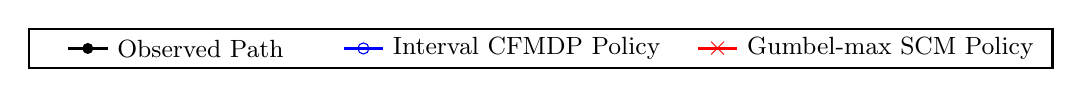
\begin{tikzpicture}[scale=1.0, every node/.style={scale=1.0}]
            \draw[thick, black] (-3, -0.25) rectangle (10, 0.25);
            %
            \draw[black, line width=1pt] (-2.5, 0.0) -- (-2,0.0);
            \fill[black] (-2.25,0.0) circle (2pt); %
            \node[right] at (-2,0.0) {\small Observed Path};
            
            %
            \draw[blue, line width=1pt] (1.0,0.0) -- (1.5,0.0);
            \node[draw=blue, circle, minimum size=4pt, inner sep=0pt] at (1.25,0.0) {}; %
            \node[right] at (1.5,0.0) {\small Interval CFMDP Policy};
            
            %
            \draw[red, line width=1pt] (5.5,0) -- (6,0);
            \node[red] at (5.75,0) {$\boldsymbol{\times}$}; %
            \node[right] at (6,0) {\small Gumbel-max SCM Policy};
        \end{tikzpicture}
    }\\
    \subfigure[\footnotesize Lowest cumulative reward: Interval CFMDP ($8000$), Gumbel-max SCM ($8000$)]{%
         \resizebox{0.76\columnwidth}{!}{
             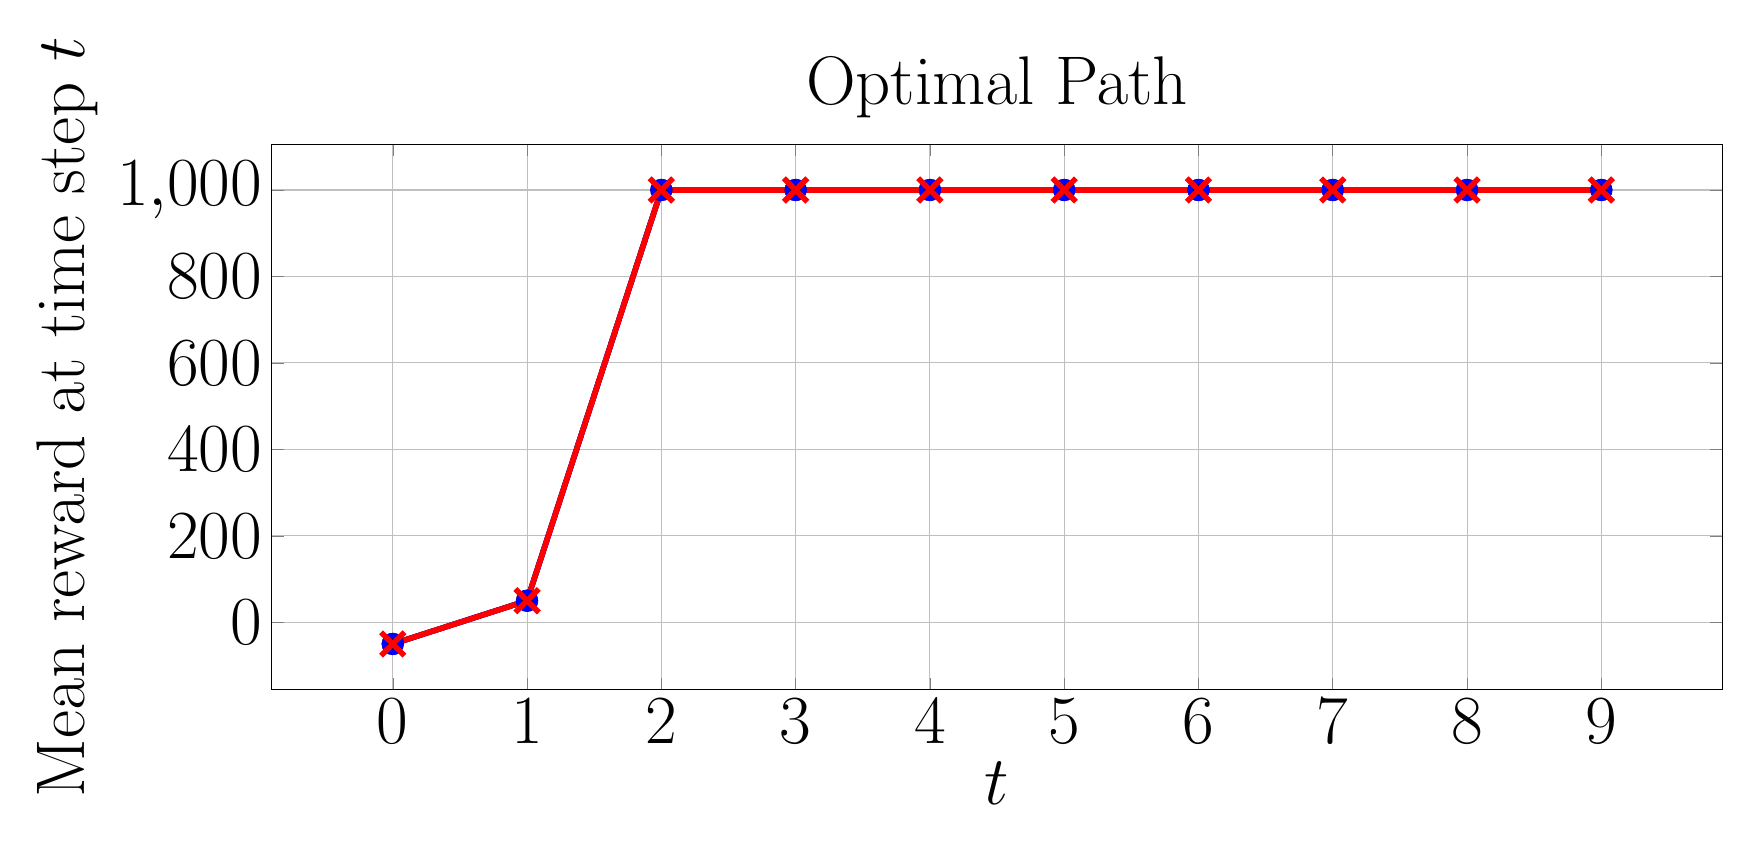
\begin{tikzpicture}
                \begin{axis}[
                    xlabel={$t$},
                    ylabel={Mean reward at time step $t$},
                    title={Optimal Path},
                    grid=both,
                    width=20cm, height=8.5cm,
                    every axis/.style={font=\Huge},
                    %
                ]
                \addplot[
                    color=black, %
                    mark=*, %
                    line width=2pt,
                    mark size=3pt,
                ]
                coordinates {
                    (0, -50.0)
                    (1, 50.0)
                    (2, 1000.0)
                    (3, 1000.0)
                    (4, 1000.0)
                    (5, 1000.0)
                    (6, 1000.0)
                    (7, 1000.0)
                    (8, 1000.0)
                    (9, 1000.0)
                };
                %
                \addplot[
                    color=blue, %
                    mark=o, %
                    line width=2pt,
                    mark size=3pt,
                    error bars/.cd,
                    y dir=both, %
                    y explicit, %
                    error bar style={line width=1pt,solid},
                    error mark options={line width=1pt,mark size=4pt,rotate=90}
                ]
                coordinates {
                    (0, -50.0)  +- (0, 0.0)
                    (1, 50.0)  +- (0, 0.0) 
                    (2, 1000.0)  +- (0, 0.0) 
                    (3, 1000.0)  +- (0, 0.0)
                    (4, 1000.0)  +- (0, 0.0)
                    (5, 1000.0) +- (0, 0.0)
                    (6, 1000.0) +- (0, 0.0)
                    (7, 1000.0) +- (0, 0.0)
                    (8, 1000.0) +- (0, 0.0)
                    (9, 1000.0) +- (0, 0.0)
                };
                %
                \addplot[
                    color=red, %
                    mark=x, %
                    line width=2pt,
                    mark size=6pt,
                    error bars/.cd,
                    y dir=both, %
                    y explicit, %
                    error bar style={line width=1pt,solid},
                    error mark options={line width=1pt,mark size=4pt,rotate=90}
                ]
                coordinates {
                    (0, -50.0)  +- (0, 0.0)
                    (1, 50.0)  +- (0, 0.0) 
                    (2, 1000.0)  +- (0, 0.0) 
                    (3, 1000.0)  +- (0, 0.0)
                    (4, 1000.0)  +- (0, 0.0)
                    (5, 1000.0) +- (0, 0.0)
                    (6, 1000.0) +- (0, 0.0)
                    (7, 1000.0) +- (0, 0.0)
                    (8, 1000.0) +- (0, 0.0)
                    (9, 1000.0) +- (0, 0.0)
                };
                %
                \end{axis}
            \end{tikzpicture}
         }
    }
    \hspace{1cm}
    \subfigure[\footnotesize Lowest cumulative reward: Interval CFMDP ($-5980$), Gumbel-max SCM ($-8000$)]{%
         \resizebox{0.76\columnwidth}{!}{
            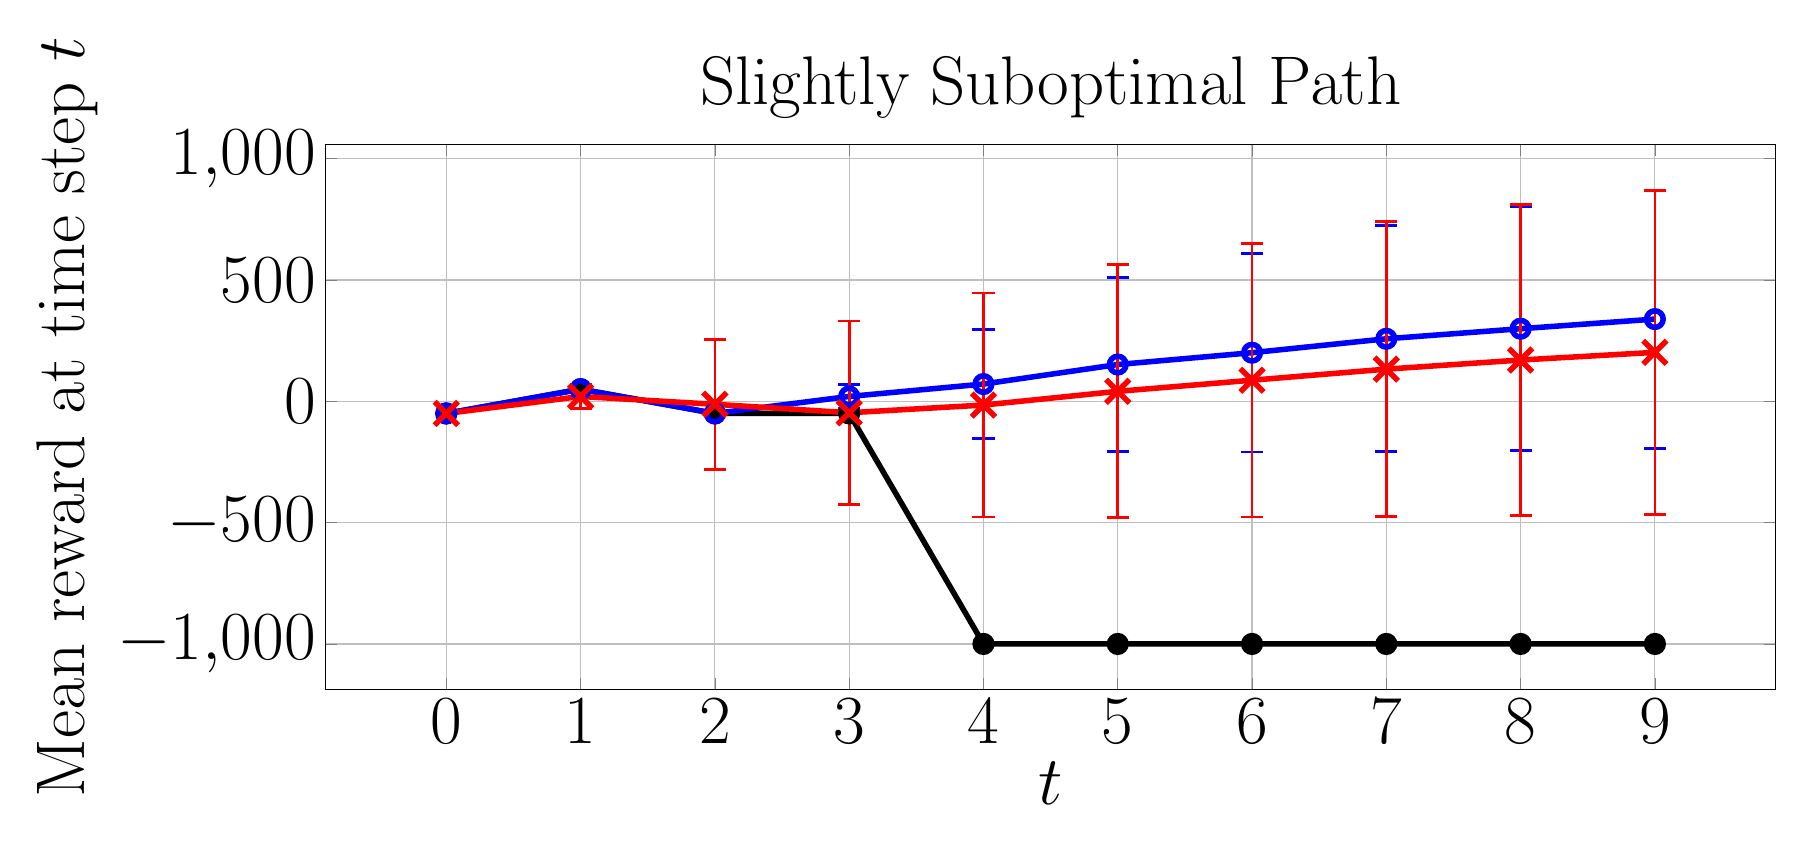
\begin{tikzpicture}
                \begin{axis}[
                    xlabel={$t$},
                    ylabel={Mean reward at time step $t$},
                    title={Slightly Suboptimal Path},
                    grid=both,
                    width=20cm, height=8.5cm,
                    every axis/.style={font=\Huge},
                    %
                ]
               \addplot[
                    color=black, %
                    mark=*, %
                    line width=2pt,
                    mark size=3pt,
                ]
                coordinates {
                    (0, -50.0)
                    (1, 50.0)
                    (2, -50.0)
                    (3, -50.0)
                    (4, -1000.0)
                    (5, -1000.0)
                    (6, -1000.0)
                    (7, -1000.0)
                    (8, -1000.0)
                    (9, -1000.0)
                };
                %
                \addplot[
                    color=blue, %
                    mark=o, %
                    line width=2pt,
                    mark size=3pt,
                    error bars/.cd,
                    y dir=both, %
                    y explicit, %
                    error bar style={line width=1pt,solid},
                    error mark options={line width=1pt,mark size=4pt,rotate=90}
                ]
                coordinates {
                    (0, -50.0)  +- (0, 0.0)
                    (1, 50.0)  +- (0, 0.0) 
                    (2, -50.0)  +- (0, 0.0) 
                    (3, 20.0631)  +- (0, 49.97539413)
                    (4, 71.206585)  +- (0, 226.02033693)
                    (5, 151.60797) +- (0, 359.23292559)
                    (6, 200.40593) +- (0, 408.86185176)
                    (7, 257.77948) +- (0, 466.10372804)
                    (8, 299.237465) +- (0, 501.82579506)
                    (9, 338.9129) +- (0, 532.06124996)
                };
                %
                \addplot[
                    color=red, %
                    mark=x, %
                    line width=2pt,
                    mark size=6pt,
                    error bars/.cd,
                    y dir=both, %
                    y explicit, %
                    error bar style={line width=1pt,solid},
                    error mark options={line width=1pt,mark size=4pt,rotate=90}
                ]
                coordinates {
                    (0, -50.0)  +- (0, 0.0)
                    (1, 20.00736)  +- (0, 49.99786741) 
                    (2, -12.282865)  +- (0, 267.598755) 
                    (3, -47.125995)  +- (0, 378.41755832)
                    (4, -15.381965)  +- (0, 461.77616558)
                    (5, 41.15459) +- (0, 521.53189262)
                    (6, 87.01595) +- (0, 564.22243126 )
                    (7, 132.62376) +- (0, 607.31338037)
                    (8, 170.168145) +- (0, 641.48013693)
                    (9, 201.813135) +- (0, 667.29441777)
                };
                %
                %
                %
                %
                %
                %
                %
                %
                %
                %
                %
                %
                %
                %
                %
                %
                %
                %
                %
                \end{axis}
            \end{tikzpicture}
         }
    }\\[-1.5pt]
    \subfigure[\footnotesize Lowest cumulative reward: Interval CFMDP ($100$), Gumbel-max SCM ($100$)]{%
         \resizebox{0.76\columnwidth}{!}{
             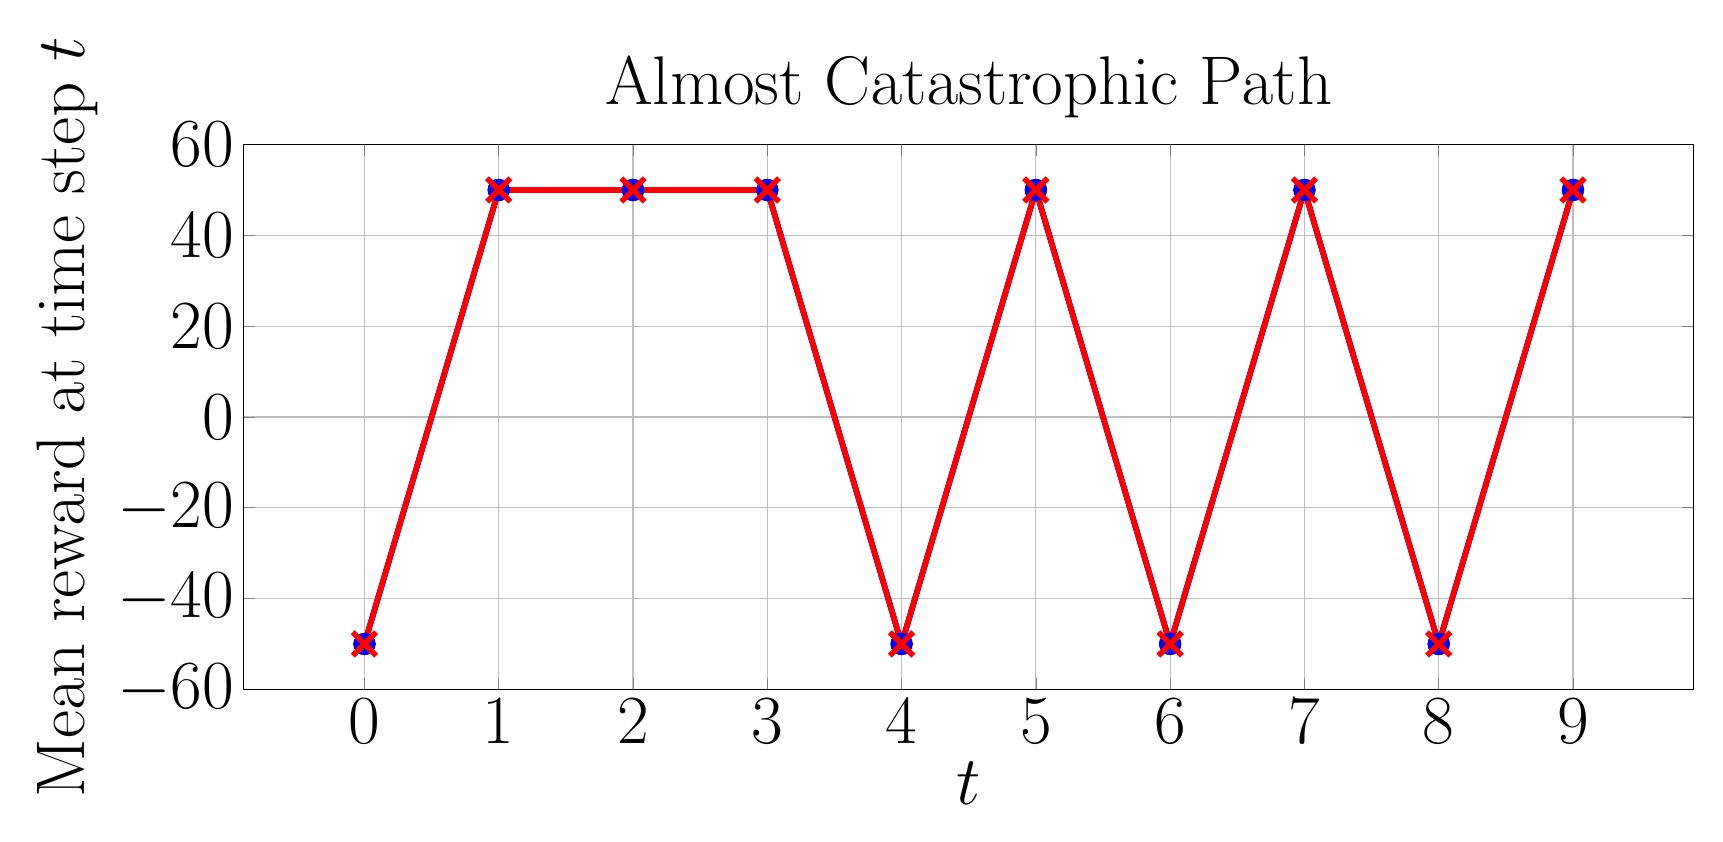
\begin{tikzpicture}
                \begin{axis}[
                    xlabel={$t$},
                    ylabel={Mean reward at time step $t$},
                    title={Almost Catastrophic Path},
                    grid=both,
                    every axis/.style={font=\Huge},
                    width=20cm, height=8.5cm,
                    %
                ]
               \addplot[
                    color=black, %
                    mark=*, %
                    line width=2pt,
                    mark size=3pt,
                ]
                coordinates {
                    (0, -50.0)
                    (1, 50.0)
                    (2, 50.0)
                    (3, 50.0)
                    (4, -50.0)
                    (5, 50.0)
                    (6, -50.0)
                    (7, 50.0)
                    (8, -50.0)
                    (9, 50.0)
                };
                %
                %
                \addplot[
                    color=blue, %
                    mark=o, %
                    line width=2pt,
                    mark size=3pt,
                    error bars/.cd,
                    y dir=both, %
                    y explicit, %
                    error bar style={line width=1pt,solid},
                    error mark options={line width=1pt,mark size=4pt,rotate=90}
                ]
                coordinates {
                    (0, -50.0)  +- (0, 0.0)
                    (1, 50.0)  +- (0, 0.0) 
                    (2, 50.0)  +- (0, 0.0) 
                    (3, 50.0)  +- (0, 0.0)
                    (4, -50.0)  +- (0, 0.0)
                    (5, 50.0) +- (0, 0.0)
                    (6, -50.0) +- (0, 0.0)
                    (7, 50.0) +- (0, 0.0)
                    (8, -50.0) +- (0, 0.0)
                    (9, 50.0) +- (0, 0.0)
                };
                %
                \addplot[
                    color=red, %
                    mark=x, %
                    line width=2pt,
                    mark size=6pt,
                    error bars/.cd,
                    y dir=both, %
                    y explicit, %
                    error bar style={line width=1pt,solid},
                    error mark options={line width=1pt,mark size=4pt,rotate=90}
                ]
                coordinates {
                    (0, -50.0)  +- (0, 0.0)
                    (1, 50.0)  +- (0, 0.0) 
                    (2, 50.0)  +- (0, 0.0) 
                    (3, 50.0)  +- (0, 0.0)
                    (4, -50.0)  +- (0, 0.0)
                    (5, 50.0) +- (0, 0.0)
                    (6, -50.0) +- (0, 0.0)
                    (7, 50.0) +- (0, 0.0)
                    (8, -50.0) +- (0, 0.0)
                    (9, 50.0) +- (0, 0.0)
                };
                %
                %
                %
                %
                %
                %
                %
                %
                %
                %
                %
                %
                %
                %
                %
                %
                %
                %
                %
                \end{axis}
            \end{tikzpicture}
         }
    }
    \hspace{1cm}
    \subfigure[\footnotesize Lowest cumulative reward: Interval CFMDP ($-7150$), Gumbel-max SCM ($-9050$)]{%
         \resizebox{0.76\columnwidth}{!}{
            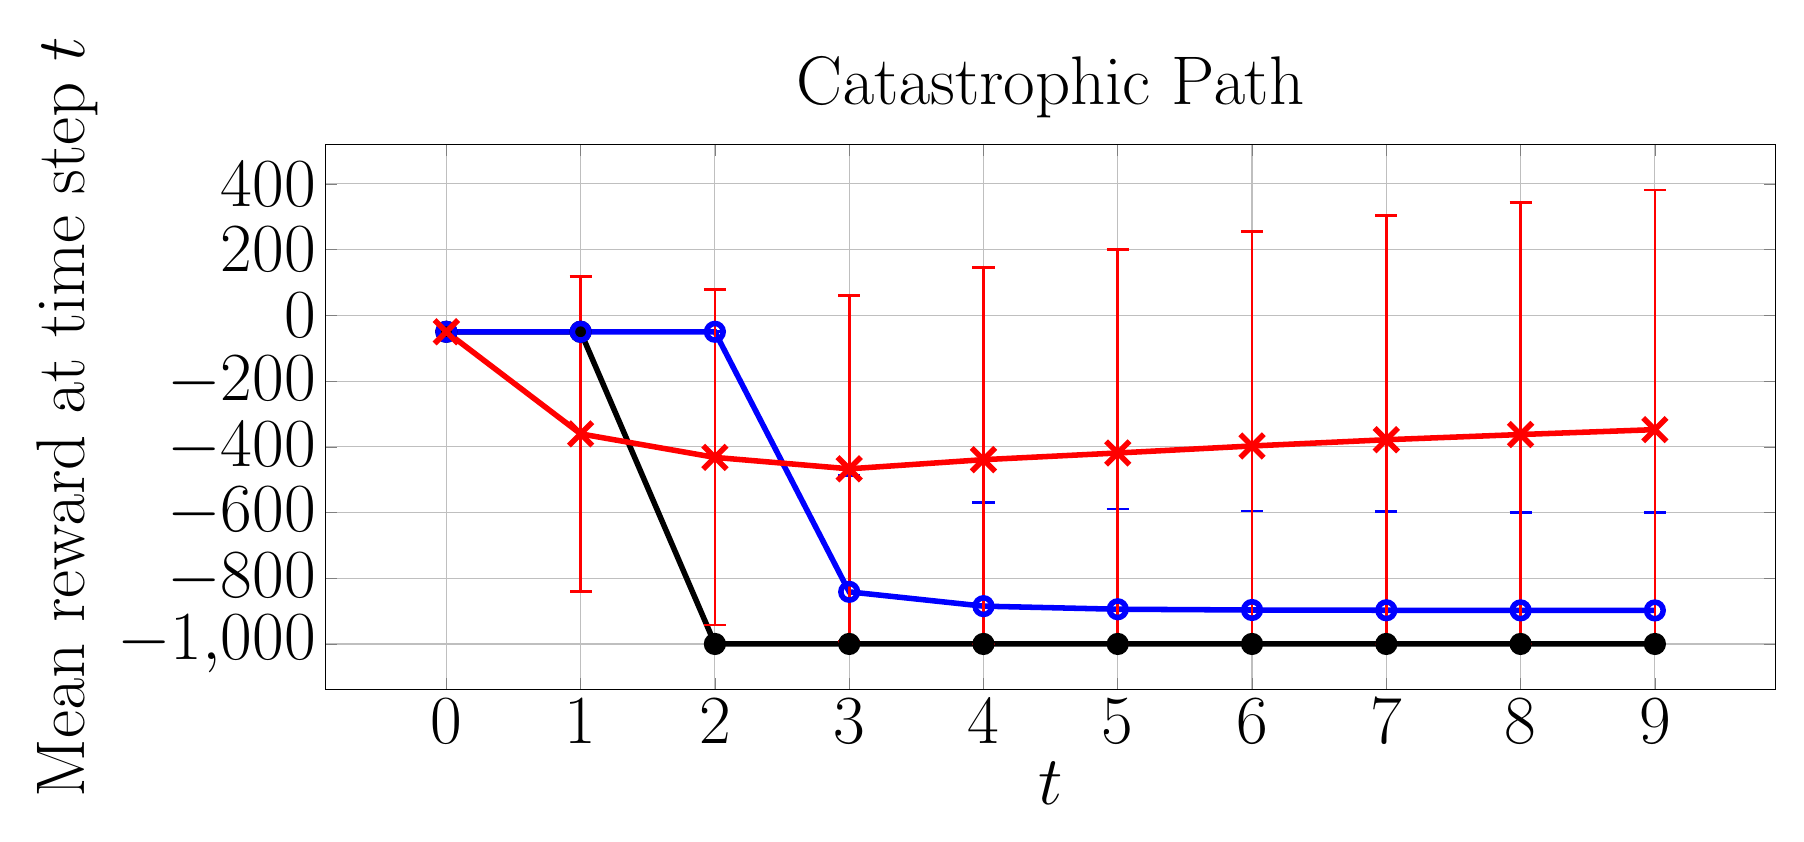
\begin{tikzpicture}
                \begin{axis}[
                    xlabel={$t$},
                    ylabel={Mean reward at time step $t$},
                    title={Catastrophic Path},
                    grid=both,
                    width=20cm, height=8.5cm,
                    every axis/.style={font=\Huge},
                    %
                ]
               \addplot[
                    color=black, %
                    mark=*, %
                    line width=2pt,
                    mark size=3pt,
                ]
                coordinates {
                    (0, -50.0)
                    (1, -50.0)
                    (2, -1000.0)
                    (3, -1000.0)
                    (4, -1000.0)
                    (5, -1000.0)
                    (6, -1000.0)
                    (7, -1000.0)
                    (8, -1000.0)
                    (9, -1000.0)
                };
                %
                %
                \addplot[
                    color=blue, %
                    mark=o, %
                    line width=2pt,
                    mark size=3pt,
                    error bars/.cd,
                    y dir=both, %
                    y explicit, %
                    error bar style={line width=1pt,solid},
                    error mark options={line width=1pt,mark size=4pt,rotate=90}
                ]
                coordinates {
                    (0, -50.0)  +- (0, 0.0)
                    (1, -50.0)  +- (0, 0.0) 
                    (2, -50.0)  +- (0, 0.0) 
                    (3, -841.440725)  += (0, 354.24605512) -= (0, 158.559275)
                    (4, -884.98225)  += (0, 315.37519669) -= (0, 115.01775)
                    (5, -894.330425) += (0, 304.88572805) -= (0, 105.669575)
                    (6, -896.696175) += (0, 301.19954514) -= (0, 103.303825)
                    (7, -897.4635) += (0, 299.61791279) -= (0, 102.5365)
                    (8, -897.77595) += (0, 298.80392585) -= (0, 102.22405)
                    (9, -897.942975) += (0, 298.32920557) -= (0, 102.057025)
                };
                %
                \addplot[
                    color=red, %
                    mark=x, %
                    line width=2pt,
                    mark size=6pt,
                    error bars/.cd,
                    y dir=both, %
                    y explicit, %
                    error bar style={line width=1pt,solid},
                    error mark options={line width=1pt,mark size=4pt,rotate=90}
                ]
            coordinates {
                    (0, -50.0)  +- (0, 0.0)
                    (1, -360.675265)  +- (0, 479.39812699) 
                    (2, -432.27629)  +- (0, 510.38620897) 
                    (3, -467.029545)  += (0, 526.36009628) -= (0, 526.36009628)
                    (4, -439.17429)  += (0, 583.96638919) -= (0, 560.82571)
                    (5, -418.82704) += (0, 618.43027478) -= (0, 581.17296)
                    (6, -397.464895) += (0, 652.67322574) -= (0, 602.535105)
                    (7, -378.49052) += (0, 682.85407033) -= (0, 621.50948)
                    (8, -362.654195) += (0, 707.01412023) -= (0, 637.345805)
                    (9, -347.737935) += (0, 729.29076479) -= (0, 652.262065)
                };
                %
                %
                %
                %
                %
                %
                %
                %
                %
                %
                %
                %
                %
                %
                %
                %
                %
                %
                %
                \end{axis}
            \end{tikzpicture}
         }
    }
    \caption{Average instant reward of CF paths induced by policies on Sepsis.}
    \label{fig: reward sepsis}
\end{figure*}

%
%
%
\subsection{Interval CFMDP Bounds}
%
%
Table \ref{tab:nonzero_probs} presents the mean counterfactual probability bound widths (excluding transitions where the upper bound is $0$) for each MDP, averaged over 20 observed paths. We compare the bounds under counterfactual stability (CS) and monotonicity (M) assumptions, CS alone, and no assumptions. This shows that the assumptions marginally reduce the bound widths, indicating the assumptions tighten the bounds without excluding too many causal models, as intended.
\renewcommand{\arraystretch}{1}

\begin{table}
\centering
\caption{Mean width of counterfactual probability bounds}
\resizebox{0.8\columnwidth}{!}{%
\begin{tabular}{|c|c|c|c|}
\hline
\multirow{2}{*}{\textbf{Environment}} & \multicolumn{3}{c|}{\textbf{Assumptions}} \\ \cline{2-4}
 & \textbf{CS + M} & \textbf{CS} & \textbf{None\tablefootnote{\jl{Equivalent to \citet{li2024probabilities}'s bounds (see Section \ref{sec: equivalence with Li}).}}} \\ \hline
\textbf{GridWorld} ($p=0.9$) & 0.0817 & 0.0977 & 0.100 \\ \hline
\textbf{GridWorld} ($p=0.4$) & 0.552  & 0.638  & 0.646 \\ \hline
\textbf{Sepsis} & 0.138 & 0.140 & 0.140 \\ \hline
\end{tabular}
}
\label{tab:nonzero_probs}
\end{table}


\subsection{Execution Times}
Table \ref{tab: times} compares the average time needed to generate the interval CFMDP vs.\ the Gumbel-max SCM CFMDP for 20 observations.
The GridWorld algorithms were run single-threaded, while the Sepsis experiments were run in parallel.
Generating the interval CFMDP is significantly faster as it uses exact analytical bounds, whereas the Gumbel-max CFMDP requires sampling from the Gumbel distribution to estimate counterfactual transition probabilities. \jl{Since constructing the counterfactual MDP models is the main bottleneck in both approaches, ours is more efficient overall and suitable for larger MDPs.}
\begin{table}
\centering
\caption{Mean execution time to generate CFMDPs}
\resizebox{0.99\columnwidth}{!}{%
\begin{tabular}{|c|c|c|}
\hline
\multirow{2}{*}{\textbf{Environment}} & \multicolumn{2}{c|}{\textbf{Mean Execution Time (s)}} \\ \cline{2-3} 
                                      & \textbf{Interval CFMDP} & \textbf{Gumbel-max CFMDP} \\ \hline
\textbf{GridWorld ($p=0.9$) }                  & 0.261                   & 56.1                      \\ \hline
\textbf{GridWorld ($p=0.4$)  }                 & 0.336                   & 54.5                      \\ \hline
\textbf{Sepsis}                                 & 688                     & 2940                      \\ \hline
\end{tabular}%
}
\label{tab: times}
\end{table}


\section{Related Work}
\textbf{Program synthesis} has been a significant area of research, with various approaches proposed to generate programs efficiently. Traditional methods, such as Transit \cite{transit} and Escher \cite{escher}, rely on bottom-up enumerative synthesis, systematically exploring the program space to identify correct solutions. Brahma \cite{loopfree} introduces an efficient SMT-based encoding for synthesizing straight-line programs that involve multiple assignments to intermediate variables. Component-based synthesizers, such as SyPet \cite{sypet}, focus on generating Java programs from examples by leveraging arbitrary libraries. However, SyPet is limited to synthesizing sequences of method calls and does not support control structures like loops or conditionals. Similarly, Python-based synthesizers such as SnipPy \cite{snippy}, CodeHint \cite{codehint}, TFCoder \cite{tfcoder}, AutoPandas \cite{autopandas}, and Wrex \cite{wrex} primarily target one-liners or sequences of method calls. These tools also provide limited support for control structures, restricting their applicability for more complex program synthesis tasks. While these methods demonstrate the potential of automated program synthesis, their limitations in handling intricate control structures underline the need for more versatile approaches.

\textbf{Synthesis with control structures.} EdSynth \cite{Edsynth} address this by lazily initializing candidates during the execution of provided tests. The execution of partially completed candidates determines the generation of future candidates, making EdSynth particularly effective for synthesis tasks that involve multiple API sequences in both the conditions and bodies of loops or branches.
FrAngel \cite{frangel} is another notable tool that supports component-based synthesis for Java programs with control structures. Unlike many traditional methods, FrAngel relies on function-level specifications and, in principle, does not require users to have a detailed understanding of the algorithm or intermediate variables. However, in practice, to make the synthesis process feasible, users must provide a variety of examples, including base and corner cases. This requirement still necessitates some level of algorithmic knowledge, and FrAngel’s relatively slow performance makes it less suitable for interactive scenarios.
LooPy \cite{loopy}, introduces the concept of an Intermediate State Graph (ISG), which compactly represents a vast space of code snippets composed of multiple assignment statements and conditionals. By engaging the programmer as an oracle to address incomplete parts of the loop, LooPy achieves a balance between automation and interactivity. Its ability to solve a wide range of synthesis tasks at interactive speeds makes it a practical tool for use cases requiring real-time feedback and adjustments.
These tools demonstrate progress in addressing the challenges of synthesis with control structures, but they also highlight trade-offs between usability, required user input, and performance.

\textbf{Large Language Models (LLMs)} have recently shown effectiveness in various software development tasks, including program synthesis\cite{jain2022jigsaw} and test generation\cite{xia2024fuzz4all,jiang2024generating}. By associating document text with code from a large training set, LLMs can generate program code from natural language prompts\cite{jain2022jigsaw,ugare2024improving,spiess2024quality,wang2023large}. Reusable API\cite{reuseableAPI} uses LLMs to generate APIs from code snippets collected from Stack Overflow and shows significant results in identifying API parameters and return types. However, they provide all the code needed and only require LLMs to create new APIs using existing implementations. Test-driven program synthesis remains an under-researched topic. How well do LLMs perform in generating entire APIs with just a few input/output examples that even end users can easily prepare? In this paper, we explore the application of LLMs in generating API implementations and finds that LLMs are effective in understanding test cases and generating viable APIs. We also show that LLMs are able to generate accurate APIs even with an incomplete set of test cases, which is very convenient. To the best of our knowledge, our work is the first systematic study of using LLMs with prompt engineering to synthesis complex APIs.

% \section{Threat to Validity}

\section{Conclusion}
In this paper, we present a novel approach of using large language models (LLMs) in API synthesis.  LLMs offer a foundational technology to capture developer insights and provide an ideal framework for enabling more effective API synthesis. The experimental results show that our approach overall outperforms FrAngel, a state-of-the-art API synthesis tool. Furthermore, our approach produces clear, maintainable code with meaningful variable names and relevant comments. Using minimal user output, our approach offers an easier way for API synthesis. We believe LLMs provide a very useful foundation for tackling the problem of complex API synthesis.






%
% ---- Bibliography ----
%
% BibTeX users should specify bibliography style 'splncs04'.
% References will then be sorted and formatted in the correct style.

\bibliographystyle{splncs04}
\bibliography{main}



% \section{First Section}
% \subsection{A Subsection Sample}
% Please note that the first paragraph of a section or subsection is
% not indented. The first paragraph that follows a table, figure,
% equation etc. does not need an indent, either.

% Subsequent paragraphs, however, are indented.

% \subsubsection{Sample Heading (Third Level)} Only two levels of
% headings should be numbered. Lower level headings remain unnumbered;
% they are formatted as run-in headings.

% \paragraph{Sample Heading (Fourth Level)}
% The contribution should contain no more than four levels of
% headings. Table~\ref{tab1} gives a summary of all heading levels.

% \begin{table}
% \caption{Table captions should be placed above the
% tables.}\label{tab1}
% \begin{tabular}{|l|l|l|}
% \hline
% Heading level &  Example & Font size and style\\
% \hline
% Title (centered) &  {\Large\bfseries Lecture Notes} & 14 point, bold\\
% 1st-level heading &  {\large\bfseries 1 Introduction} & 12 point, bold\\
% 2nd-level heading & {\bfseries 2.1 Printing Area} & 10 point, bold\\
% 3rd-level heading & {\bfseries Run-in Heading in Bold.} Text follows & 10 point, bold\\
% 4th-level heading & {\itshape Lowest Level Heading.} Text follows & 10 point, italic\\
% \hline
% \end{tabular}
% \end{table}


% \noindent Displayed equations are centered and set on a separate
% line.
% \begin{equation}
% x + y = z
% \end{equation}
% Please try to avoid rasterized images for line-art diagrams and
% schemas. Whenever possible, use vector graphics instead (see
% Fig.~\ref{fig1}).

% \begin{figure}
% \includegraphics[width=\textwidth]{fig1.eps}
% \caption{A figure caption is always placed below the illustration.
% Please note that short captions are centered, while long ones are
% justified by the macro package automatically.} \label{fig1}
% \end{figure}

% \begin{theorem}
% This is a sample theorem. The run-in heading is set in bold, while
% the following text appears in italics. Definitions, lemmas,
% propositions, and corollaries are styled the same way.
% \end{theorem}
% %
% % the environments 'definition', 'lemma', 'proposition', 'corollary',
% % 'remark', and 'example' are defined in the LLNCS documentclass as well.
% %
% \begin{proof}
% Proofs, examples, and remarks have the initial word in italics,
% while the following text appears in normal font.
% \end{proof}
% For citations of references, we prefer the use of square brackets
% and consecutive numbers. Citations using labels or the author/year
% convention are also acceptable. The following bibliography provides
% a sample reference list with entries for journal
% articles~\cite{ref_article1}, an LNCS chapter~\cite{ref_lncs1}, a
% book~\cite{ref_book1}, proceedings without editors~\cite{ref_proc1},
% and a homepage~\cite{ref_url1}. Multiple citations are grouped
% \cite{ref_article1,ref_lncs1,ref_book1},
% \cite{ref_article1,ref_book1,ref_proc1,ref_url1}.

% \begin{credits}
% \subsubsection{\ackname} A bold run-in heading in small font size at the end of the paper is
% used for general acknowledgments, for example: This study was funded
% by X (grant number Y).

% \subsubsection{\discintname}
% It is now necessary to declare any competing interests or to specifically
% state that the authors have no competing interests. Please place the
% statement with a bold run-in heading in small font size beneath the
% (optional) acknowledgments\footnote{If EquinOCS, our proceedings submission
% system, is used, then the disclaimer can be provided directly in the system.},
% for example: The authors have no competing interests to declare that are
% relevant to the content of this article. Or: Author A has received research
% grants from Company W. Author B has received a speaker honorarium from
% Company X and owns stock in Company Y. Author C is a member of committee Z.
% \end{credits}

\appendix
\section{Prompt}
\begin{figure}
	\centering
\begin{lstlisting}[style = prompt]
<Role>
    You are a software engineer. You will be given with an Java method signature,
    its return type, and a set of test cases as comments. Your task is to implement
    the Java method into a full implementation to pass the test cases.
</Role>
<Instruction>
    Use the following step by step instruction to solve the problem:
        Step 1 - Import Necessary Libraries
            (1) Identify and include any required import statements, such as Java standard libraries (java.util.*), or open-source libraries (e.g., Apache Commons, Guava) to simplify implementation.
            (2) Ensure that all dependencies are properly referenced to facilitate a smooth compilation.
        Step 2 - Define Any Required Helper Classes or Methods
            (1) If the method requires additional data structures or utility functions, define them before implementing the main method.
            (2) Ensure helper classes or methods are designed efficiently to support modularity and reusability.
        Step 3 - Create a Public Class with an Appropriate Name
            (1) Define a class that logically represents the method's functionality (e.g., APIUtility, StringProcessor, MathHelper).
            (2) Ensure the class is structured according to Java best practices.
        Step 4 - Understand the Problem Statement and Requirements
            (1) Analyze the method signature, return type, and test cases to infer the expected behavior.
            (2) Identify edge cases that may not be explicitly covered by the test cases but are crucial for correctness (e.g., null inputs, empty lists, boundary values).
        Step 5 - Implement the Method to Pass All Test Cases
            (1) Write a clear and efficient implementation of the method to meet the expected input-output requirements.
            (2) Optimize for performance and maintainability while ensuring correctness.
        Step 6 - Validate Edge Cases and Complete Implementation
            (1) Consider additional edge cases beyond the provided test cases (e.g., large inputs, invalid values).
            (2) Refactor the code if necessary to handle all identified cases.
        Step 7 - Write Unit Tests for Each Provided Test Case
            (1) Create a test method for each given test case using JUnit (or another testing framework).
            (2) Ensure test methods cover normal, edge, and erroneous inputs.
        Step 8 - Provide a Main Method for Execution and Validation
            (1) Implement a main method to run and validate the test cases.
            (2) Print test results to confirm correctness and ensure all test cases pass.
            (3) Verify that the code compiles and runs without errors.
</Instruction>
<examples> 
    Here is one example:
    <method>
        List<Integer> GetRange(int start, int end)
    </method>
    <TestCases>
        1. start = 10, end = 9 -> output: []
        2. start = 10, end = 10 -> output: []
        3. start = 10, end = 11 -> output: [10]
        4. start = 10, end = 12 -> output: [10, 11]
        5. start = -2, end = 2 -> output: [-2, -1, 0, 1]
    </TestCases>
    <output>
        List<Integer> GetRange(int start, int end) {
            ArrayList<Integer> range = new ArrayList<Integer>();
            for (int i=0; i+start < end; i++)
                range.add(Integer.valueOf(i+start));
            return range
        }
    </output>
</examples>
Now, give you the following method signature and test cases:
<method>
     double ellipseArea(Ellipse2D ellipse)
</method>
<TestCases>
    1.  Ellipse2D.Double(12.3, -45.6, 7.8, 9) -> 3.9 * 4.5 * Math.PI
    2.  Ellipse2D.Double(12.3, -45.6, 7.8, 2) -> 3.9 * Math.PI
    3.  Ellipse2D.Double(12.3, -45.6, 2, 7.8) -> 3.9 * Math.PI
    4.  Ellipse2D.Double(12.3, -45.6, 2, 2) -> Math.PI
</TestCases>

Please output the results. Only output complete code.
 \end{lstlisting}
 \caption{An example of our prompt input to LLMs}
		\label{fig:figure4}
\end{figure}

\end{document}
